% Options for packages loaded elsewhere
\PassOptionsToPackage{unicode}{hyperref}
\PassOptionsToPackage{hyphens}{url}
\PassOptionsToPackage{dvipsnames,svgnames,x11names}{xcolor}
%
\documentclass[
  letterpaper,
  DIV=11,
  numbers=noendperiod]{scrreprt}

\usepackage{amsmath,amssymb}
\usepackage{lmodern}
\usepackage{iftex}
\ifPDFTeX
  \usepackage[T1]{fontenc}
  \usepackage[utf8]{inputenc}
  \usepackage{textcomp} % provide euro and other symbols
\else % if luatex or xetex
  \usepackage{unicode-math}
  \defaultfontfeatures{Scale=MatchLowercase}
  \defaultfontfeatures[\rmfamily]{Ligatures=TeX,Scale=1}
\fi
% Use upquote if available, for straight quotes in verbatim environments
\IfFileExists{upquote.sty}{\usepackage{upquote}}{}
\IfFileExists{microtype.sty}{% use microtype if available
  \usepackage[]{microtype}
  \UseMicrotypeSet[protrusion]{basicmath} % disable protrusion for tt fonts
}{}
\makeatletter
\@ifundefined{KOMAClassName}{% if non-KOMA class
  \IfFileExists{parskip.sty}{%
    \usepackage{parskip}
  }{% else
    \setlength{\parindent}{0pt}
    \setlength{\parskip}{6pt plus 2pt minus 1pt}}
}{% if KOMA class
  \KOMAoptions{parskip=half}}
\makeatother
\usepackage{xcolor}
\setlength{\emergencystretch}{3em} % prevent overfull lines
\setcounter{secnumdepth}{5}
% Make \paragraph and \subparagraph free-standing
\ifx\paragraph\undefined\else
  \let\oldparagraph\paragraph
  \renewcommand{\paragraph}[1]{\oldparagraph{#1}\mbox{}}
\fi
\ifx\subparagraph\undefined\else
  \let\oldsubparagraph\subparagraph
  \renewcommand{\subparagraph}[1]{\oldsubparagraph{#1}\mbox{}}
\fi

\usepackage{color}
\usepackage{fancyvrb}
\newcommand{\VerbBar}{|}
\newcommand{\VERB}{\Verb[commandchars=\\\{\}]}
\DefineVerbatimEnvironment{Highlighting}{Verbatim}{commandchars=\\\{\}}
% Add ',fontsize=\small' for more characters per line
\usepackage{framed}
\definecolor{shadecolor}{RGB}{241,243,245}
\newenvironment{Shaded}{\begin{snugshade}}{\end{snugshade}}
\newcommand{\AlertTok}[1]{\textcolor[rgb]{0.68,0.00,0.00}{#1}}
\newcommand{\AnnotationTok}[1]{\textcolor[rgb]{0.37,0.37,0.37}{#1}}
\newcommand{\AttributeTok}[1]{\textcolor[rgb]{0.40,0.45,0.13}{#1}}
\newcommand{\BaseNTok}[1]{\textcolor[rgb]{0.68,0.00,0.00}{#1}}
\newcommand{\BuiltInTok}[1]{\textcolor[rgb]{0.00,0.23,0.31}{#1}}
\newcommand{\CharTok}[1]{\textcolor[rgb]{0.13,0.47,0.30}{#1}}
\newcommand{\CommentTok}[1]{\textcolor[rgb]{0.37,0.37,0.37}{#1}}
\newcommand{\CommentVarTok}[1]{\textcolor[rgb]{0.37,0.37,0.37}{\textit{#1}}}
\newcommand{\ConstantTok}[1]{\textcolor[rgb]{0.56,0.35,0.01}{#1}}
\newcommand{\ControlFlowTok}[1]{\textcolor[rgb]{0.00,0.23,0.31}{#1}}
\newcommand{\DataTypeTok}[1]{\textcolor[rgb]{0.68,0.00,0.00}{#1}}
\newcommand{\DecValTok}[1]{\textcolor[rgb]{0.68,0.00,0.00}{#1}}
\newcommand{\DocumentationTok}[1]{\textcolor[rgb]{0.37,0.37,0.37}{\textit{#1}}}
\newcommand{\ErrorTok}[1]{\textcolor[rgb]{0.68,0.00,0.00}{#1}}
\newcommand{\ExtensionTok}[1]{\textcolor[rgb]{0.00,0.23,0.31}{#1}}
\newcommand{\FloatTok}[1]{\textcolor[rgb]{0.68,0.00,0.00}{#1}}
\newcommand{\FunctionTok}[1]{\textcolor[rgb]{0.28,0.35,0.67}{#1}}
\newcommand{\ImportTok}[1]{\textcolor[rgb]{0.00,0.46,0.62}{#1}}
\newcommand{\InformationTok}[1]{\textcolor[rgb]{0.37,0.37,0.37}{#1}}
\newcommand{\KeywordTok}[1]{\textcolor[rgb]{0.00,0.23,0.31}{#1}}
\newcommand{\NormalTok}[1]{\textcolor[rgb]{0.00,0.23,0.31}{#1}}
\newcommand{\OperatorTok}[1]{\textcolor[rgb]{0.37,0.37,0.37}{#1}}
\newcommand{\OtherTok}[1]{\textcolor[rgb]{0.00,0.23,0.31}{#1}}
\newcommand{\PreprocessorTok}[1]{\textcolor[rgb]{0.68,0.00,0.00}{#1}}
\newcommand{\RegionMarkerTok}[1]{\textcolor[rgb]{0.00,0.23,0.31}{#1}}
\newcommand{\SpecialCharTok}[1]{\textcolor[rgb]{0.37,0.37,0.37}{#1}}
\newcommand{\SpecialStringTok}[1]{\textcolor[rgb]{0.13,0.47,0.30}{#1}}
\newcommand{\StringTok}[1]{\textcolor[rgb]{0.13,0.47,0.30}{#1}}
\newcommand{\VariableTok}[1]{\textcolor[rgb]{0.07,0.07,0.07}{#1}}
\newcommand{\VerbatimStringTok}[1]{\textcolor[rgb]{0.13,0.47,0.30}{#1}}
\newcommand{\WarningTok}[1]{\textcolor[rgb]{0.37,0.37,0.37}{\textit{#1}}}

\providecommand{\tightlist}{%
  \setlength{\itemsep}{0pt}\setlength{\parskip}{0pt}}\usepackage{longtable,booktabs,array}
\usepackage{calc} % for calculating minipage widths
% Correct order of tables after \paragraph or \subparagraph
\usepackage{etoolbox}
\makeatletter
\patchcmd\longtable{\par}{\if@noskipsec\mbox{}\fi\par}{}{}
\makeatother
% Allow footnotes in longtable head/foot
\IfFileExists{footnotehyper.sty}{\usepackage{footnotehyper}}{\usepackage{footnote}}
\makesavenoteenv{longtable}
\usepackage{graphicx}
\makeatletter
\def\maxwidth{\ifdim\Gin@nat@width>\linewidth\linewidth\else\Gin@nat@width\fi}
\def\maxheight{\ifdim\Gin@nat@height>\textheight\textheight\else\Gin@nat@height\fi}
\makeatother
% Scale images if necessary, so that they will not overflow the page
% margins by default, and it is still possible to overwrite the defaults
% using explicit options in \includegraphics[width, height, ...]{}
\setkeys{Gin}{width=\maxwidth,height=\maxheight,keepaspectratio}
% Set default figure placement to htbp
\makeatletter
\def\fps@figure{htbp}
\makeatother
\newlength{\cslhangindent}
\setlength{\cslhangindent}{1.5em}
\newlength{\csllabelwidth}
\setlength{\csllabelwidth}{3em}
\newlength{\cslentryspacingunit} % times entry-spacing
\setlength{\cslentryspacingunit}{\parskip}
\newenvironment{CSLReferences}[2] % #1 hanging-ident, #2 entry spacing
 {% don't indent paragraphs
  \setlength{\parindent}{0pt}
  % turn on hanging indent if param 1 is 1
  \ifodd #1
  \let\oldpar\par
  \def\par{\hangindent=\cslhangindent\oldpar}
  \fi
  % set entry spacing
  \setlength{\parskip}{#2\cslentryspacingunit}
 }%
 {}
\usepackage{calc}
\newcommand{\CSLBlock}[1]{#1\hfill\break}
\newcommand{\CSLLeftMargin}[1]{\parbox[t]{\csllabelwidth}{#1}}
\newcommand{\CSLRightInline}[1]{\parbox[t]{\linewidth - \csllabelwidth}{#1}\break}
\newcommand{\CSLIndent}[1]{\hspace{\cslhangindent}#1}

\usepackage{booktabs}
\usepackage{longtable}
\usepackage{array}
\usepackage{multirow}
\usepackage{wrapfig}
\usepackage{float}
\usepackage{colortbl}
\usepackage{pdflscape}
\usepackage{tabu}
\usepackage{threeparttable}
\usepackage{threeparttablex}
\usepackage[normalem]{ulem}
\usepackage{makecell}
\usepackage{xcolor}
\KOMAoption{captions}{tableheading}
\makeatletter
\@ifpackageloaded{tcolorbox}{}{\usepackage[many]{tcolorbox}}
\@ifpackageloaded{fontawesome5}{}{\usepackage{fontawesome5}}
\definecolor{quarto-callout-color}{HTML}{909090}
\definecolor{quarto-callout-note-color}{HTML}{0758E5}
\definecolor{quarto-callout-important-color}{HTML}{CC1914}
\definecolor{quarto-callout-warning-color}{HTML}{EB9113}
\definecolor{quarto-callout-tip-color}{HTML}{00A047}
\definecolor{quarto-callout-caution-color}{HTML}{FC5300}
\definecolor{quarto-callout-color-frame}{HTML}{acacac}
\definecolor{quarto-callout-note-color-frame}{HTML}{4582ec}
\definecolor{quarto-callout-important-color-frame}{HTML}{d9534f}
\definecolor{quarto-callout-warning-color-frame}{HTML}{f0ad4e}
\definecolor{quarto-callout-tip-color-frame}{HTML}{02b875}
\definecolor{quarto-callout-caution-color-frame}{HTML}{fd7e14}
\makeatother
\makeatletter
\makeatother
\makeatletter
\@ifpackageloaded{bookmark}{}{\usepackage{bookmark}}
\makeatother
\makeatletter
\@ifpackageloaded{caption}{}{\usepackage{caption}}
\AtBeginDocument{%
\ifdefined\contentsname
  \renewcommand*\contentsname{Table of contents}
\else
  \newcommand\contentsname{Table of contents}
\fi
\ifdefined\listfigurename
  \renewcommand*\listfigurename{List of Figures}
\else
  \newcommand\listfigurename{List of Figures}
\fi
\ifdefined\listtablename
  \renewcommand*\listtablename{List of Tables}
\else
  \newcommand\listtablename{List of Tables}
\fi
\ifdefined\figurename
  \renewcommand*\figurename{Figure}
\else
  \newcommand\figurename{Figure}
\fi
\ifdefined\tablename
  \renewcommand*\tablename{Table}
\else
  \newcommand\tablename{Table}
\fi
}
\@ifpackageloaded{float}{}{\usepackage{float}}
\floatstyle{ruled}
\@ifundefined{c@chapter}{\newfloat{codelisting}{h}{lop}}{\newfloat{codelisting}{h}{lop}[chapter]}
\floatname{codelisting}{Listing}
\newcommand*\listoflistings{\listof{codelisting}{List of Listings}}
\makeatother
\makeatletter
\@ifpackageloaded{caption}{}{\usepackage{caption}}
\@ifpackageloaded{subcaption}{}{\usepackage{subcaption}}
\makeatother
\makeatletter
\@ifpackageloaded{tcolorbox}{}{\usepackage[many]{tcolorbox}}
\makeatother
\makeatletter
\@ifundefined{shadecolor}{\definecolor{shadecolor}{rgb}{.97, .97, .97}}
\makeatother
\makeatletter
\makeatother
\ifLuaTeX
  \usepackage{selnolig}  % disable illegal ligatures
\fi
\IfFileExists{bookmark.sty}{\usepackage{bookmark}}{\usepackage{hyperref}}
\IfFileExists{xurl.sty}{\usepackage{xurl}}{} % add URL line breaks if available
\urlstyle{same} % disable monospaced font for URLs
\hypersetup{
  pdftitle={INF511: Modern Regression I},
  pdfauthor={Joseph Mihaljevic, PhD; Isaac Shaffer, MS},
  colorlinks=true,
  linkcolor={blue},
  filecolor={Maroon},
  citecolor={Blue},
  urlcolor={Blue},
  pdfcreator={LaTeX via pandoc}}

\title{INF511: Modern Regression I}
\usepackage{etoolbox}
\makeatletter
\providecommand{\subtitle}[1]{% add subtitle to \maketitle
  \apptocmd{\@title}{\par {\large #1 \par}}{}{}
}
\makeatother
\subtitle{Spring 2023}
\author{Joseph Mihaljevic, PhD \and Isaac Shaffer, MS}
\date{}

\begin{document}
\maketitle
\ifdefined\Shaded\renewenvironment{Shaded}{\begin{tcolorbox}[enhanced, sharp corners, borderline west={3pt}{0pt}{shadecolor}, interior hidden, frame hidden, boxrule=0pt, breakable]}{\end{tcolorbox}}\fi

\renewcommand*\contentsname{Table of contents}
{
\hypersetup{linkcolor=}
\setcounter{tocdepth}{2}
\tableofcontents
}
\bookmarksetup{startatroot}

\hypertarget{preface}{%
\chapter*{Preface}\label{preface}}
\addcontentsline{toc}{chapter}{Preface}

\markboth{Preface}{Preface}

Welcome to INF511: Modern Regression I. In this course, we will do a
deep dive into three fundamental methods for estimating the linear
relationships between random variables (i.e., linear regression
analysis): ordinary least squares (Chapter~\ref{sec-ols}), maximum
likelihood (Chapter~\ref{sec-max-lik}), and Bayesian inference
(Chapter~\ref{sec-bayesian}). We will also explore null hypothesis
testing (Chapter~\ref{sec-hypothesis}), and linear models with
categorical covariates (i.e., ANOVA, Chapter~\ref{sec-anova}). This
online book serves as a living document of resources for our class. The
chapters provide links to lecture materials, which should be downloaded
and printed prior to class, as well as links to recorded lectures. Each
chapter also has material that is supplemental to lecture, with coded
examples. We will often refer to these examples during class time, and
they will be helpful for solving problem set and homework assignments.
Problem sets will have dedicated in-class time, whereas homework
assignments will be conducted entirely outside of class time.

Please refer to the Syllabus (Appendix~\ref{sec-syllabus}) for the
course schedule, learning objectives, grading structure, course
policies, etc.

\hypertarget{footnotes}{%
\section*{Footnotes}\label{footnotes}}
\addcontentsline{toc}{section}{Footnotes}

\markright{Footnotes}

\begin{itemize}
\tightlist
\item
  This is a Quarto book. To learn more about Quarto books visit
  \url{https://quarto.org/docs/books}.
\item
  This website is published using
  \href{https://pages.github.com/}{Github Pages}.
\item
  See Knuth (1984) for additional discussion of literate programming.
\end{itemize}

\part{Pre-requisites}

\hypertarget{software}{%
\chapter{Software}\label{software}}

You will need to have all of the following free software downloaded and
in working order on your laptop.

\begin{tcolorbox}[enhanced jigsaw, colback=white, title=\textcolor{quarto-callout-important-color}{\faExclamation}\hspace{0.5em}{Prior to first lecture}, left=2mm, coltitle=black, bottomrule=.15mm, arc=.35mm, toprule=.15mm, rightrule=.15mm, opacityback=0, opacitybacktitle=0.6, colframe=quarto-callout-important-color-frame, leftrule=.75mm, toptitle=1mm, titlerule=0mm, breakable, bottomtitle=1mm, colbacktitle=quarto-callout-important-color!10!white]

You must have the following on your laptops prior to the first lecture.

\end{tcolorbox}

\begin{itemize}
\tightlist
\item
  Latest version of \href{https://posit.co/downloads/}{RStudio Desktop
  IDE}
\item
  Compatible version of \href{https://ftp.osuosl.org/pub/cran/}{R
  software environment}
\item
  \href{https://quarto.org/docs/get-started/}{Quarto} publishing system
  (for documents with integrated code).
\item
  You must have a functional PDF Engine to render Quarto (\texttt{.qmd})
  documents into PDF. See this section on
  \href{https://quarto.org/docs/output-formats/pdf-engine.html}{PDF
  Engines}, and be sure to test whether you can render an example
  \texttt{.qmd} file into a PDF.
\end{itemize}

\begin{tcolorbox}[enhanced jigsaw, colback=white, title=\textcolor{quarto-callout-important-color}{\faExclamation}\hspace{0.5em}{Prior to Bayesian inference}, left=2mm, coltitle=black, bottomrule=.15mm, arc=.35mm, toprule=.15mm, rightrule=.15mm, opacityback=0, opacitybacktitle=0.6, colframe=quarto-callout-important-color-frame, leftrule=.75mm, toptitle=1mm, titlerule=0mm, breakable, bottomtitle=1mm, colbacktitle=quarto-callout-important-color!10!white]

You must have the following on your laptops prior to the sections on
Bayesian inference.

\end{tcolorbox}

\begin{itemize}
\tightlist
\item
  Stan programming language, via the
  \href{https://mc-stan.org/users/interfaces/rstan.html}{rstan} package
  for R.
\item
  We will potentially use the R package \texttt{rstanarm}, but this is a
  straightforward package to download using the
  \texttt{install.packages()} function.
\end{itemize}

\hypertarget{sec-Rintro}{%
\chapter{Introduction to R}\label{sec-Rintro}}

This Appendix serves two purposes. First, it introduces you to R.
Second, it introduces functions for conducting an ordinary least squares
(OLS) regression on a data set supplied within R.

The nice thing about Quarto (similar to .RMD) files, is that you can
integrate code within text files. The text files can be rendered into
HTML, PDF, or Word documents (among others). These documents are
therefore like a `laboratory' notebook that allow you to show your
coding work, visual outputs, and contextualizing your work with text
using a visually aesthetic framework.

R is a free and open-source programming language, with many functions
supplied by the ``base'' code. However, many other functions require
loading 3rd party packages. Be aware that none of the functions in these
other packages are guaranteed to work in a certain way (although many
are very well maintained and validated by large user bases). You'll need
to do your own research to make sure which functions can be trusted, and
sometimes you'll need to devise your own strategies to test the
functions to make sure they work as they claim to.

\hypertarget{load-a-package}{%
\section{Load a package}\label{load-a-package}}

\begin{Shaded}
\begin{Highlighting}[]
\CommentTok{\# The library() function loads R packages that are not supplied in the "base" software}
\CommentTok{\# You need to install a package once before loading}
\CommentTok{\# install.packages(\textquotesingle{}dplyr\textquotesingle{})}
\CommentTok{\# Load the \textquotesingle{}dplyr\textquotesingle{} package which has many convenient data manipulation functions}
\FunctionTok{library}\NormalTok{(dplyr) }
\end{Highlighting}
\end{Shaded}

\hypertarget{load-a-data-set}{%
\section{Load a data set}\label{load-a-data-set}}

\begin{Shaded}
\begin{Highlighting}[]
\CommentTok{\# R has many built{-}in data sets for educational purposes.}
\CommentTok{\# The data() function will show all of these, with descriptions}
\FunctionTok{data}\NormalTok{() }\CommentTok{\# Do this on your own.}
\end{Highlighting}
\end{Shaded}

\hypertarget{manipulate-and-visualize-the-data}{%
\section{Manipulate and visualize the
data}\label{manipulate-and-visualize-the-data}}

\begin{Shaded}
\begin{Highlighting}[]
\CommentTok{\# Load the \textquotesingle{}iris\textquotesingle{} data set, which contains lengths and widths of flower petals}
\CommentTok{\# We choose this, because these lengths and widths are often linearly associated}
\FunctionTok{data}\NormalTok{(iris)}

\FunctionTok{is.data.frame}\NormalTok{(iris) }\CommentTok{\# Validate as data frame object}
\end{Highlighting}
\end{Shaded}

\begin{verbatim}
[1] TRUE
\end{verbatim}

\begin{Shaded}
\begin{Highlighting}[]
\FunctionTok{is.vector}\NormalTok{(iris) }\CommentTok{\# Not a vector object}
\end{Highlighting}
\end{Shaded}

\begin{verbatim}
[1] FALSE
\end{verbatim}

\begin{Shaded}
\begin{Highlighting}[]
\FunctionTok{str}\NormalTok{(iris) }\CommentTok{\# Show general object characteristics}
\end{Highlighting}
\end{Shaded}

\begin{verbatim}
'data.frame':   150 obs. of  5 variables:
 $ Sepal.Length: num  5.1 4.9 4.7 4.6 5 5.4 4.6 5 4.4 4.9 ...
 $ Sepal.Width : num  3.5 3 3.2 3.1 3.6 3.9 3.4 3.4 2.9 3.1 ...
 $ Petal.Length: num  1.4 1.4 1.3 1.5 1.4 1.7 1.4 1.5 1.4 1.5 ...
 $ Petal.Width : num  0.2 0.2 0.2 0.2 0.2 0.4 0.3 0.2 0.2 0.1 ...
 $ Species     : Factor w/ 3 levels "setosa","versicolor",..: 1 1 1 1 1 1 1 1 1 1 ...
\end{verbatim}

\begin{Shaded}
\begin{Highlighting}[]
\FunctionTok{glimpse}\NormalTok{(iris) }\CommentTok{\# Similar to str() but more detailed/relevant}
\end{Highlighting}
\end{Shaded}

\begin{verbatim}
Rows: 150
Columns: 5
$ Sepal.Length <dbl> 5.1, 4.9, 4.7, 4.6, 5.0, 5.4, 4.6, 5.0, 4.4, 4.9, 5.4, 4.~
$ Sepal.Width  <dbl> 3.5, 3.0, 3.2, 3.1, 3.6, 3.9, 3.4, 3.4, 2.9, 3.1, 3.7, 3.~
$ Petal.Length <dbl> 1.4, 1.4, 1.3, 1.5, 1.4, 1.7, 1.4, 1.5, 1.4, 1.5, 1.5, 1.~
$ Petal.Width  <dbl> 0.2, 0.2, 0.2, 0.2, 0.2, 0.4, 0.3, 0.2, 0.2, 0.1, 0.2, 0.~
$ Species      <fct> setosa, setosa, setosa, setosa, setosa, setosa, setosa, s~
\end{verbatim}

\begin{Shaded}
\begin{Highlighting}[]
\CommentTok{\# glimpse() is a function within the dplyr package. }
\CommentTok{\# We can call the function like this, because dplyr was loaded already}
\CommentTok{\# Alternatively we can use the following syntax to call non{-}base functions}
\NormalTok{dplyr}\SpecialCharTok{::}\FunctionTok{glimpse}\NormalTok{(iris)}
\end{Highlighting}
\end{Shaded}

\begin{verbatim}
Rows: 150
Columns: 5
$ Sepal.Length <dbl> 5.1, 4.9, 4.7, 4.6, 5.0, 5.4, 4.6, 5.0, 4.4, 4.9, 5.4, 4.~
$ Sepal.Width  <dbl> 3.5, 3.0, 3.2, 3.1, 3.6, 3.9, 3.4, 3.4, 2.9, 3.1, 3.7, 3.~
$ Petal.Length <dbl> 1.4, 1.4, 1.3, 1.5, 1.4, 1.7, 1.4, 1.5, 1.4, 1.5, 1.5, 1.~
$ Petal.Width  <dbl> 0.2, 0.2, 0.2, 0.2, 0.2, 0.4, 0.3, 0.2, 0.2, 0.1, 0.2, 0.~
$ Species      <fct> setosa, setosa, setosa, setosa, setosa, setosa, setosa, s~
\end{verbatim}

\begin{Shaded}
\begin{Highlighting}[]
\CommentTok{\# This way, you are less prone to errors, especially if }
\CommentTok{\# functions in different packages are named the same or similarly (masking)}
\end{Highlighting}
\end{Shaded}

From the \texttt{glimpse()} function we see that there are five columns
within the \texttt{iris} data frame, and there are 150 total data points
(rows). We also see that four columns are numeric doubles, while one
(Species) is a factor.

\begin{Shaded}
\begin{Highlighting}[]
\CommentTok{\# Subset column vectors from the data frame using the \textquotesingle{}$\textquotesingle{} symbol}
\FunctionTok{mean}\NormalTok{(iris}\SpecialCharTok{$}\NormalTok{Petal.Length)}
\end{Highlighting}
\end{Shaded}

\begin{verbatim}
[1] 3.758
\end{verbatim}

\begin{Shaded}
\begin{Highlighting}[]
\CommentTok{\# R can do \textquotesingle{}vectorized\textquotesingle{} functions }
\NormalTok{iris}\SpecialCharTok{$}\NormalTok{Petal.Width }\SpecialCharTok{*} \DecValTok{2}
\end{Highlighting}
\end{Shaded}

\begin{verbatim}
  [1] 0.4 0.4 0.4 0.4 0.4 0.8 0.6 0.4 0.4 0.2 0.4 0.4 0.2 0.2 0.4 0.8 0.8 0.6
 [19] 0.6 0.6 0.4 0.8 0.4 1.0 0.4 0.4 0.8 0.4 0.4 0.4 0.4 0.8 0.2 0.4 0.4 0.4
 [37] 0.4 0.2 0.4 0.4 0.6 0.6 0.4 1.2 0.8 0.6 0.4 0.4 0.4 0.4 2.8 3.0 3.0 2.6
 [55] 3.0 2.6 3.2 2.0 2.6 2.8 2.0 3.0 2.0 2.8 2.6 2.8 3.0 2.0 3.0 2.2 3.6 2.6
 [73] 3.0 2.4 2.6 2.8 2.8 3.4 3.0 2.0 2.2 2.0 2.4 3.2 3.0 3.2 3.0 2.6 2.6 2.6
 [91] 2.4 2.8 2.4 2.0 2.6 2.4 2.6 2.6 2.2 2.6 5.0 3.8 4.2 3.6 4.4 4.2 3.4 3.6
[109] 3.6 5.0 4.0 3.8 4.2 4.0 4.8 4.6 3.6 4.4 4.6 3.0 4.6 4.0 4.0 3.6 4.2 3.6
[127] 3.6 3.6 4.2 3.2 3.8 4.0 4.4 3.0 2.8 4.6 4.8 3.6 3.6 4.2 4.8 4.6 3.8 4.6
[145] 5.0 4.6 3.8 4.0 4.6 3.6
\end{verbatim}

\begin{Shaded}
\begin{Highlighting}[]
\CommentTok{\# Check if factor}
\FunctionTok{is.factor}\NormalTok{(iris}\SpecialCharTok{$}\NormalTok{Species)}
\end{Highlighting}
\end{Shaded}

\begin{verbatim}
[1] TRUE
\end{verbatim}

\begin{Shaded}
\begin{Highlighting}[]
\FunctionTok{is.character}\NormalTok{(iris}\SpecialCharTok{$}\NormalTok{Species)}
\end{Highlighting}
\end{Shaded}

\begin{verbatim}
[1] FALSE
\end{verbatim}

Let's make some exploratory visualizations.

\begin{Shaded}
\begin{Highlighting}[]
\CommentTok{\# Histogram}
\FunctionTok{hist}\NormalTok{(iris}\SpecialCharTok{$}\NormalTok{Petal.Length)}
\FunctionTok{hist}\NormalTok{(iris}\SpecialCharTok{$}\NormalTok{Petal.Width)}
\end{Highlighting}
\end{Shaded}

\begin{figure}

\begin{minipage}[t]{0.50\linewidth}

{\centering 

\raisebox{-\height}{

\includegraphics{./Rintro_files/figure-pdf/unnamed-chunk-10-1.pdf}

}

}

\end{minipage}%
%
\begin{minipage}[t]{0.50\linewidth}

{\centering 

\raisebox{-\height}{

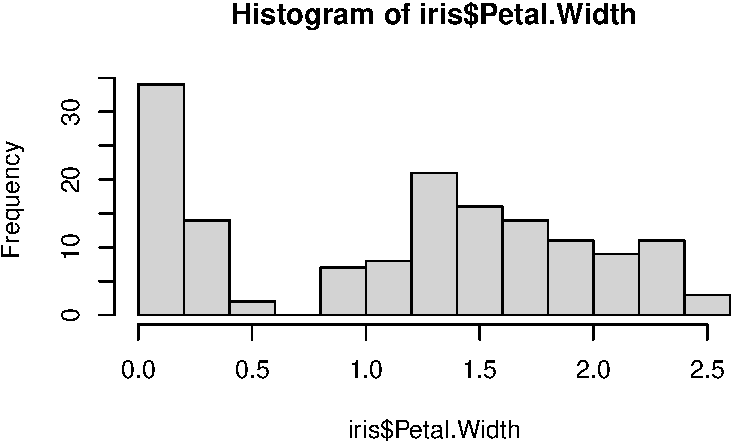
\includegraphics{./Rintro_files/figure-pdf/unnamed-chunk-10-2.pdf}

}

}

\end{minipage}%

\end{figure}

\begin{Shaded}
\begin{Highlighting}[]
\CommentTok{\# Explore association between random variables}
\CommentTok{\# formula method: y \textasciitilde{} x }
\CommentTok{\# Read the above like: }
\CommentTok{\# y{-}variable \textquotesingle{}modeled by\textquotesingle{} x{-}variable, or}
\CommentTok{\# y{-}variable \textquotesingle{}as a function of\textquotesingle{} x{-}variable}
\FunctionTok{plot}\NormalTok{(iris}\SpecialCharTok{$}\NormalTok{Petal.Width }\SpecialCharTok{\textasciitilde{}}\NormalTok{ iris}\SpecialCharTok{$}\NormalTok{Petal.Length,}
     \AttributeTok{xlab =} \StringTok{"Length"}\NormalTok{,}
     \AttributeTok{ylab =} \StringTok{"Width"}\NormalTok{,}
     \AttributeTok{pch =} \DecValTok{19}\NormalTok{) }\CommentTok{\#pch = plot character}
\end{Highlighting}
\end{Shaded}

\begin{figure}[H]

{\centering \includegraphics{./Rintro_files/figure-pdf/unnamed-chunk-12-1.pdf}

}

\end{figure}

\hypertarget{is-there-a-linear-association}{%
\section{Is there a linear
association?}\label{is-there-a-linear-association}}

The goal of regression is to determine the functional association
between random variables. With linear regression the specific goal is to
test whether there is a linear relationship between a response variable
(\emph{y}) and one or more covariates (\emph{x}). The form of the
functional relationship is:
\[y_i = \beta_0 + \beta_1 x_i + \epsilon_i ,\] where \(y_i\) is the
\(i\)-th data point, \(\beta_0\) is the intercept, \(\beta_1\) is the
slope, and \(x\) is the single covariate in the model. In matrix form we
have: \[\bf{y} = \bf{X} \bf{B} + \boldsymbol\epsilon\] For hypothesis
testing, we are testing the null hypothesis that the slope of the
relationship between \(x\) and \(y\) is zero (i.e., no detectable linear
relationship, \(\beta_1 = 0\)).

We can conduct linear regression in R using the \texttt{lm()} function,
where `lm' stands for `linear model'. This function specifically
estimates the model parameter (slope, intercept, and residual variance),
using the ordinary least squares approach, which we will soon learn in
lecture.

\begin{Shaded}
\begin{Highlighting}[]
\NormalTok{my\_model }\OtherTok{=} \FunctionTok{lm}\NormalTok{(}\AttributeTok{formula =}\NormalTok{ Petal.Width }\SpecialCharTok{\textasciitilde{}}\NormalTok{ Petal.Length,}
              \AttributeTok{data =}\NormalTok{ iris)}
\end{Highlighting}
\end{Shaded}

The line above stores the output of the linear model in the
\texttt{my\_model} object. We can then manipulate the \texttt{my\_model}
object and apply various functions to help us understand the outcome of
the linear regression analysis.

\begin{Shaded}
\begin{Highlighting}[]
\FunctionTok{str}\NormalTok{(my\_model)}
\end{Highlighting}
\end{Shaded}

\begin{verbatim}
List of 12
 $ coefficients : Named num [1:2] -0.363 0.416
  ..- attr(*, "names")= chr [1:2] "(Intercept)" "Petal.Length"
 $ residuals    : Named num [1:150] -0.019 -0.019 0.0226 -0.0606 -0.019 ...
  ..- attr(*, "names")= chr [1:150] "1" "2" "3" "4" ...
 $ effects      : Named num [1:150] -14.6888 8.9588 0.0257 -0.0576 -0.0159 ...
  ..- attr(*, "names")= chr [1:150] "(Intercept)" "Petal.Length" "" "" ...
 $ rank         : int 2
 $ fitted.values: Named num [1:150] 0.219 0.219 0.177 0.261 0.219 ...
  ..- attr(*, "names")= chr [1:150] "1" "2" "3" "4" ...
 $ assign       : int [1:2] 0 1
 $ qr           :List of 5
  ..$ qr   : num [1:150, 1:2] -12.2474 0.0816 0.0816 0.0816 0.0816 ...
  .. ..- attr(*, "dimnames")=List of 2
  .. .. ..$ : chr [1:150] "1" "2" "3" "4" ...
  .. .. ..$ : chr [1:2] "(Intercept)" "Petal.Length"
  .. ..- attr(*, "assign")= int [1:2] 0 1
  ..$ qraux: num [1:2] 1.08 1.1
  ..$ pivot: int [1:2] 1 2
  ..$ tol  : num 1e-07
  ..$ rank : int 2
  ..- attr(*, "class")= chr "qr"
 $ df.residual  : int 148
 $ xlevels      : Named list()
 $ call         : language lm(formula = Petal.Width ~ Petal.Length, data = iris)
 $ terms        :Classes 'terms', 'formula'  language Petal.Width ~ Petal.Length
  .. ..- attr(*, "variables")= language list(Petal.Width, Petal.Length)
  .. ..- attr(*, "factors")= int [1:2, 1] 0 1
  .. .. ..- attr(*, "dimnames")=List of 2
  .. .. .. ..$ : chr [1:2] "Petal.Width" "Petal.Length"
  .. .. .. ..$ : chr "Petal.Length"
  .. ..- attr(*, "term.labels")= chr "Petal.Length"
  .. ..- attr(*, "order")= int 1
  .. ..- attr(*, "intercept")= int 1
  .. ..- attr(*, "response")= int 1
  .. ..- attr(*, ".Environment")=<environment: R_GlobalEnv> 
  .. ..- attr(*, "predvars")= language list(Petal.Width, Petal.Length)
  .. ..- attr(*, "dataClasses")= Named chr [1:2] "numeric" "numeric"
  .. .. ..- attr(*, "names")= chr [1:2] "Petal.Width" "Petal.Length"
 $ model        :'data.frame':  150 obs. of  2 variables:
  ..$ Petal.Width : num [1:150] 0.2 0.2 0.2 0.2 0.2 0.4 0.3 0.2 0.2 0.1 ...
  ..$ Petal.Length: num [1:150] 1.4 1.4 1.3 1.5 1.4 1.7 1.4 1.5 1.4 1.5 ...
  ..- attr(*, "terms")=Classes 'terms', 'formula'  language Petal.Width ~ Petal.Length
  .. .. ..- attr(*, "variables")= language list(Petal.Width, Petal.Length)
  .. .. ..- attr(*, "factors")= int [1:2, 1] 0 1
  .. .. .. ..- attr(*, "dimnames")=List of 2
  .. .. .. .. ..$ : chr [1:2] "Petal.Width" "Petal.Length"
  .. .. .. .. ..$ : chr "Petal.Length"
  .. .. ..- attr(*, "term.labels")= chr "Petal.Length"
  .. .. ..- attr(*, "order")= int 1
  .. .. ..- attr(*, "intercept")= int 1
  .. .. ..- attr(*, "response")= int 1
  .. .. ..- attr(*, ".Environment")=<environment: R_GlobalEnv> 
  .. .. ..- attr(*, "predvars")= language list(Petal.Width, Petal.Length)
  .. .. ..- attr(*, "dataClasses")= Named chr [1:2] "numeric" "numeric"
  .. .. .. ..- attr(*, "names")= chr [1:2] "Petal.Width" "Petal.Length"
 - attr(*, "class")= chr "lm"
\end{verbatim}

Obviously, the output of the analysis is a complicated data structure
with many elements. There are, however, some convenient functions to
summarize these outputs for us.

\begin{Shaded}
\begin{Highlighting}[]
\FunctionTok{summary}\NormalTok{(my\_model)}
\end{Highlighting}
\end{Shaded}

\begin{verbatim}

Call:
lm(formula = Petal.Width ~ Petal.Length, data = iris)

Residuals:
     Min       1Q   Median       3Q      Max 
-0.56515 -0.12358 -0.01898  0.13288  0.64272 

Coefficients:
              Estimate Std. Error t value Pr(>|t|)    
(Intercept)  -0.363076   0.039762  -9.131  4.7e-16 ***
Petal.Length  0.415755   0.009582  43.387  < 2e-16 ***
---
Signif. codes:  0 '***' 0.001 '**' 0.01 '*' 0.05 '.' 0.1 ' ' 1

Residual standard error: 0.2065 on 148 degrees of freedom
Multiple R-squared:  0.9271,    Adjusted R-squared:  0.9266 
F-statistic:  1882 on 1 and 148 DF,  p-value: < 2.2e-16
\end{verbatim}

Above is the main outcome that we care about. The \texttt{summary()}
function tells us the parameter estimates (with estimates of parameter
uncertainty). It also conducts null-hypothesis testing, providing
p-values, and shows the goodness of model fit, using R-squared.

\begin{tcolorbox}[enhanced jigsaw, colback=white, title=\textcolor{quarto-callout-tip-color}{\faLightbulb}\hspace{0.5em}{Tip}, left=2mm, coltitle=black, bottomrule=.15mm, arc=.35mm, toprule=.15mm, rightrule=.15mm, opacityback=0, opacitybacktitle=0.6, colframe=quarto-callout-tip-color-frame, leftrule=.75mm, toptitle=1mm, titlerule=0mm, breakable, bottomtitle=1mm, colbacktitle=quarto-callout-tip-color!10!white]

The goal of the first part of this course is to understand in sufficient
detail how this analysis is conducted, so that we can interpret the
results from a well-informed standpoint.

\end{tcolorbox}

\begin{Shaded}
\begin{Highlighting}[]
\FunctionTok{plot}\NormalTok{(iris}\SpecialCharTok{$}\NormalTok{Petal.Width }\SpecialCharTok{\textasciitilde{}}\NormalTok{ iris}\SpecialCharTok{$}\NormalTok{Petal.Length,}
     \AttributeTok{xlab =} \StringTok{"Length"}\NormalTok{,}
     \AttributeTok{ylab =} \StringTok{"Width"}\NormalTok{,}
     \AttributeTok{pch =} \DecValTok{19}\NormalTok{)}
\CommentTok{\# Add the estimated linear relationship}
\FunctionTok{abline}\NormalTok{(}\AttributeTok{reg =}\NormalTok{ my\_model)}
\end{Highlighting}
\end{Shaded}

\begin{figure}[H]

{\centering \includegraphics{./Rintro_files/figure-pdf/unnamed-chunk-20-1.pdf}

}

\caption{Data with fitted linear relationship.}

\end{figure}

\hypertarget{probability-distributions}{%
\chapter{Probability distributions}\label{probability-distributions}}

\hypertarget{lecture-material}{%
\section{Lecture material}\label{lecture-material}}

Please download and print the lecture material from here. After lecture,
the recording will also appear in this section.

\hypertarget{gaussian-normal-distribution}{%
\section{Gaussian (Normal)
distribution}\label{gaussian-normal-distribution}}

As we learned in lecture, the normal distribution is defined by two
parameters, the mean \(\mu\) and the standard deviation \(\sigma\).
Here, we will use the normal distribution to demonstrate some of R's
functions to describe probability distributions and to draw random
numbers from probability distributions. Let's assume that random
variable \(x\) follows a normal distribution,
\(x_i \sim N(\mu, \sigma)\).

\begin{Shaded}
\begin{Highlighting}[]
\CommentTok{\# Define the parameters}
\NormalTok{mu }\OtherTok{=} \DecValTok{10}
\NormalTok{sigma }\OtherTok{=} \FloatTok{2.5}

\CommentTok{\# Visualize the probability density function (pdf)}
\NormalTok{x\_vals }\OtherTok{=} \FunctionTok{seq}\NormalTok{(}\DecValTok{0}\NormalTok{, }\DecValTok{50}\NormalTok{, }\AttributeTok{by =} \FloatTok{0.1}\NormalTok{)}
\NormalTok{norm\_pdf }\OtherTok{=} \FunctionTok{dnorm}\NormalTok{(x\_vals, }\AttributeTok{mean =}\NormalTok{ mu, }\AttributeTok{sd =}\NormalTok{ sigma)}

\CommentTok{\# Let\textquotesingle{}s use some of the other R functions to describe the distribution}

\DocumentationTok{\#\# What is the probability density of specific values?}
\DocumentationTok{\#\# mean}
\NormalTok{p\_mu }\OtherTok{=} \FunctionTok{dnorm}\NormalTok{(mu, }\AttributeTok{mean =}\NormalTok{ mu, }\AttributeTok{sd =}\NormalTok{ sigma)}
\DocumentationTok{\#\# The next two values will describe the 95\% probability density bounds}
\DocumentationTok{\#\# (Low) 2.5\% cut off }
\NormalTok{x\_low95 }\OtherTok{=} \FunctionTok{qnorm}\NormalTok{(}\FloatTok{0.025}\NormalTok{, }\AttributeTok{mean =}\NormalTok{ mu, }\AttributeTok{sd =}\NormalTok{ sigma)}
\NormalTok{p\_low95 }\OtherTok{=} \FunctionTok{dnorm}\NormalTok{(x\_low95, }\AttributeTok{mean =}\NormalTok{ mu, }\AttributeTok{sd =}\NormalTok{ sigma)}
\DocumentationTok{\#\# (High) 97.5\% cut off}
\NormalTok{x\_high95 }\OtherTok{=} \FunctionTok{qnorm}\NormalTok{(}\FloatTok{0.975}\NormalTok{, }\AttributeTok{mean =}\NormalTok{ mu, }\AttributeTok{sd =}\NormalTok{ sigma)}
\NormalTok{p\_high95 }\OtherTok{=} \FunctionTok{dnorm}\NormalTok{(x\_high95, }\AttributeTok{mean =}\NormalTok{ mu, }\AttributeTok{sd =}\NormalTok{ sigma)}

\CommentTok{\# So, what is the P(x \textless{}= x\_high95)??}
\FunctionTok{pnorm}\NormalTok{(x\_high95, }\AttributeTok{mean =}\NormalTok{ mu, }\AttributeTok{sd =}\NormalTok{ sigma)}
\end{Highlighting}
\end{Shaded}

\begin{verbatim}
[1] 0.975
\end{verbatim}

\begin{Shaded}
\begin{Highlighting}[]
\DocumentationTok{\#\# Plot the pdf with segments}
\FunctionTok{plot}\NormalTok{(}\AttributeTok{x =} \ConstantTok{NA}\NormalTok{, }\AttributeTok{y =} \ConstantTok{NA}\NormalTok{, }\AttributeTok{xlim =} \FunctionTok{c}\NormalTok{(}\DecValTok{0}\NormalTok{, }\DecValTok{20}\NormalTok{), }\AttributeTok{ylim =} \FunctionTok{c}\NormalTok{(}\DecValTok{0}\NormalTok{, }\FloatTok{0.2}\NormalTok{),}
     \AttributeTok{xlab =} \StringTok{"x"}\NormalTok{, }\AttributeTok{ylab =} \FunctionTok{expression}\NormalTok{(}\StringTok{"P(x |"}\SpecialCharTok{\textasciitilde{}}\NormalTok{mu}\SpecialCharTok{\textasciitilde{}}\StringTok{","}\SpecialCharTok{\textasciitilde{}}\NormalTok{sigma}\SpecialCharTok{\textasciitilde{}}\StringTok{")"}\NormalTok{))}
\FunctionTok{lines}\NormalTok{(norm\_pdf }\SpecialCharTok{\textasciitilde{}}\NormalTok{ x\_vals)}
\FunctionTok{segments}\NormalTok{(}\AttributeTok{x0 =} \FunctionTok{c}\NormalTok{(x\_low95, mu, x\_high95), }\AttributeTok{x1 =} \FunctionTok{c}\NormalTok{(x\_low95, mu, x\_high95),}
         \AttributeTok{y0 =} \FunctionTok{rep}\NormalTok{(}\DecValTok{0}\NormalTok{, }\AttributeTok{times =} \DecValTok{3}\NormalTok{), }\AttributeTok{y1 =} \FunctionTok{c}\NormalTok{(p\_low95, p\_mu, p\_high95))}
\CommentTok{\# Now, let\textquotesingle{}s draw random samples from this normal distribution}
\NormalTok{n\_rand }\OtherTok{=} \DecValTok{1000}
\NormalTok{x\_rand }\OtherTok{=} \FunctionTok{rnorm}\NormalTok{(n\_rand, }\AttributeTok{mean =}\NormalTok{ mu, }\AttributeTok{sd =}\NormalTok{ sigma)}

\CommentTok{\# Plot a histogram and overlay the approximate expectations}
\DocumentationTok{\#\# The line below assumes you draw \textquotesingle{}n\_rand\textquotesingle{} samples}
\FunctionTok{hist}\NormalTok{(x\_rand, }\AttributeTok{breaks =} \DecValTok{20}\NormalTok{, }\AttributeTok{main =} \StringTok{""}\NormalTok{)}
\FunctionTok{lines}\NormalTok{(norm\_pdf}\SpecialCharTok{*}\NormalTok{n\_rand }\SpecialCharTok{\textasciitilde{}}\NormalTok{ x\_vals)}
\end{Highlighting}
\end{Shaded}

\begin{figure}

\begin{minipage}[t]{0.50\linewidth}

{\centering 

\raisebox{-\height}{

\includegraphics{./prob_files/figure-pdf/unnamed-chunk-4-1.pdf}

}

}

\end{minipage}%
%
\begin{minipage}[t]{0.50\linewidth}

{\centering 

\raisebox{-\height}{

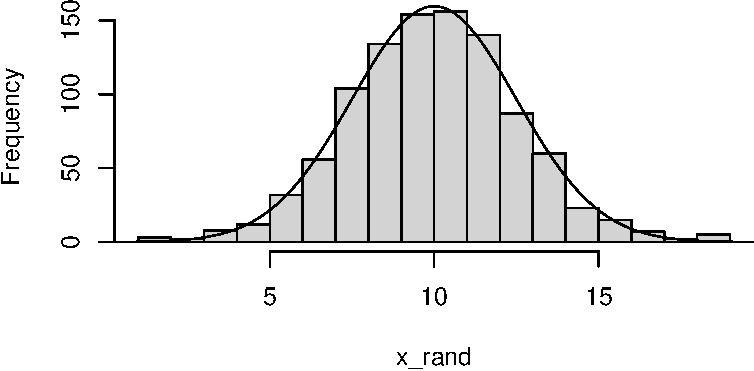
\includegraphics{./prob_files/figure-pdf/unnamed-chunk-4-2.pdf}

}

}

\end{minipage}%

\end{figure}

\hypertarget{multivariate-normal-distribution}{%
\section{Multivariate normal
distribution}\label{multivariate-normal-distribution}}

\hypertarget{relation-to-residuals-epsilon}{%
\subsection{\texorpdfstring{Relation to residuals,
\(\epsilon\)}{Relation to residuals, \textbackslash epsilon}}\label{relation-to-residuals-epsilon}}

Recall our linear model in matrix notation: \(Y = XB + \epsilon\). We
use the multivariate normal distribution to describe the probability
density of the residuals, \(\epsilon\). Recall that each individual
residual, \(\epsilon_i\) follows a normal distribution with mean zero
and standard deviation equal to the residual error, \(\sigma\):
\(\epsilon_i \sim N(0, \sigma)\). Also recall that the linear regression
analysis assumes that \(\epsilon_i\) are I.I.D. (independent and
identically distributed). \(\epsilon_i \sim N(0, \sigma)\) implies the
identical distribution (i.e., each residual follows the same normal
distribution). The ``independent'' part means that the residual values
are not correlated in any way, meaning that they do not covariance is
zero. Thus, we can use vector notation to say that the vector
\(\epsilon\) follows a multivariate normal distribution with all means
equal to zero and covariance matrix \(\Sigma = \sigma^2 I\), where \(I\)
is a square identity matrix: \(\epsilon \sim N(0, \sigma^2 I)\). More
about covariance and covariance matrices is available below
(Footnotes~\ref{sec-covariance}).

The multivariate normal probability distribution is hard to visualize,
because it is in multiple dimensions. But we can use similar R functions
to understand the distribution. These functions are not in the base
installation of R, so we need another package, \texttt{MASS}. We'll also
need the \texttt{Matrix} package later.

\begin{Shaded}
\begin{Highlighting}[]
\CommentTok{\# Install packages if you don\textquotesingle{}t already have them, e.g., }
\CommentTok{\# install.packages("MASS", dependencies = TRUE)}
\FunctionTok{library}\NormalTok{(MASS)}
\FunctionTok{library}\NormalTok{(Matrix)}

\CommentTok{\# Define mean and st.dev.}
\NormalTok{mu\_epsilon }\OtherTok{=} \DecValTok{0}
\NormalTok{sigma\_epsilon }\OtherTok{=} \FloatTok{2.0}

\CommentTok{\# sample size}
\NormalTok{n\_resid }\OtherTok{=} \DecValTok{1000}

\CommentTok{\# we need a vector of means}
\NormalTok{mu\_vec }\OtherTok{=} \FunctionTok{rep}\NormalTok{(}\DecValTok{0}\NormalTok{, n\_resid)}

\CommentTok{\# we need an identity matrix}
\NormalTok{I\_mat }\OtherTok{=} \FunctionTok{matrix}\NormalTok{(}\DecValTok{0}\NormalTok{, }\AttributeTok{nrow =}\NormalTok{ n\_resid, }\AttributeTok{ncol =}\NormalTok{ n\_resid)}
\DocumentationTok{\#\# specify the diagonal = 1}
\FunctionTok{diag}\NormalTok{(I\_mat) }\OtherTok{=} \DecValTok{1}

\CommentTok{\# Draw randomly from the multivariate normal}
\NormalTok{mvn\_epsilon }\OtherTok{=}\NormalTok{ MASS}\SpecialCharTok{::}\FunctionTok{mvrnorm}\NormalTok{(}\AttributeTok{n =} \DecValTok{1}\NormalTok{, }
                            \AttributeTok{mu =}\NormalTok{ mu\_vec,}
                            \AttributeTok{Sigma =}\NormalTok{ sigma\_epsilon}\SpecialCharTok{\^{}}\DecValTok{2}\SpecialCharTok{*}\NormalTok{I\_mat)}
\CommentTok{\# We can see that an entire array of size n\_resid is drawn}
\FunctionTok{str}\NormalTok{(mvn\_epsilon)}
\end{Highlighting}
\end{Shaded}

\begin{verbatim}
 num [1:1000] -2.921 0.177 2.471 -2.111 1.004 ...
\end{verbatim}

\begin{Shaded}
\begin{Highlighting}[]
\CommentTok{\# How does this compare to drawing them independently?}
\NormalTok{norm\_epsilon }\OtherTok{=} \FunctionTok{rnorm}\NormalTok{(n\_resid, }\AttributeTok{mean =}\NormalTok{ mu\_epsilon, }\AttributeTok{sd =}\NormalTok{ sigma\_epsilon)}
\FunctionTok{c}\NormalTok{(}\FunctionTok{mean}\NormalTok{(mvn\_epsilon), }\FunctionTok{mean}\NormalTok{(norm\_epsilon))}
\end{Highlighting}
\end{Shaded}

\begin{verbatim}
[1] -0.02419969  0.10170744
\end{verbatim}

\begin{Shaded}
\begin{Highlighting}[]
\FunctionTok{c}\NormalTok{(}\FunctionTok{sd}\NormalTok{(mvn\_epsilon), }\FunctionTok{sd}\NormalTok{(norm\_epsilon))}
\end{Highlighting}
\end{Shaded}

\begin{verbatim}
[1] 2.014499 2.020977
\end{verbatim}

\begin{Shaded}
\begin{Highlighting}[]
\CommentTok{\# Compare these two vectors visually:}
\FunctionTok{hist}\NormalTok{(mvn\_epsilon)}
\FunctionTok{hist}\NormalTok{(norm\_epsilon)}
\end{Highlighting}
\end{Shaded}

\begin{figure}

\begin{minipage}[t]{0.50\linewidth}

{\centering 

\raisebox{-\height}{

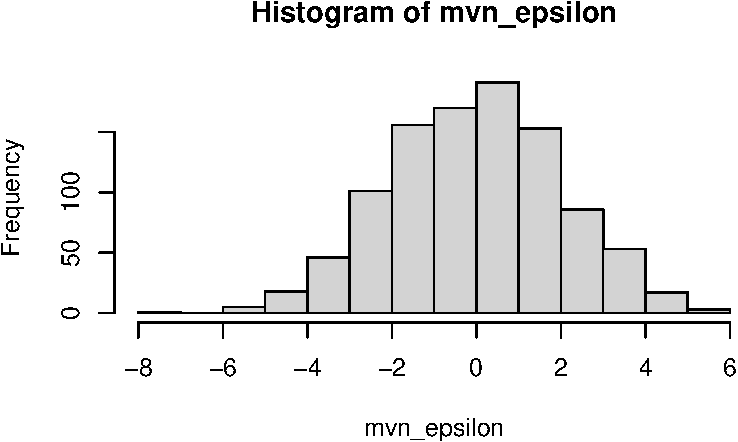
\includegraphics{./prob_files/figure-pdf/unnamed-chunk-8-1.pdf}

}

}

\end{minipage}%
%
\begin{minipage}[t]{0.50\linewidth}

{\centering 

\raisebox{-\height}{

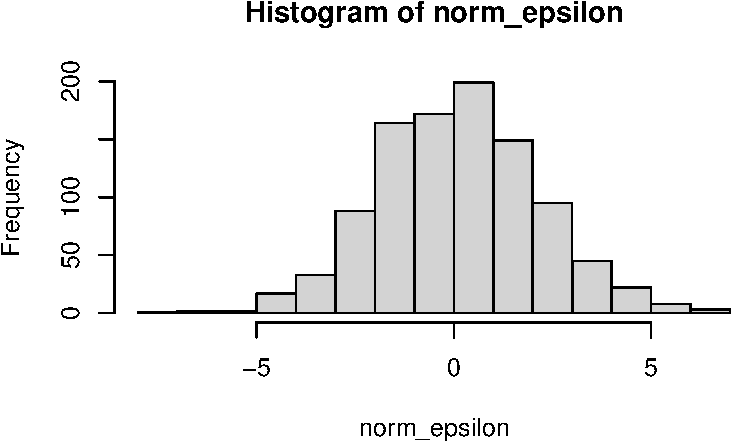
\includegraphics{./prob_files/figure-pdf/unnamed-chunk-8-2.pdf}

}

}

\end{minipage}%

\end{figure}

\hypertarget{multivariate-normal-distribution-with-non-independent-variables}{%
\subsection{Multivariate normal distribution with non-independent
variables}\label{multivariate-normal-distribution-with-non-independent-variables}}

Let's explore the multivariate normal a bit more. Suppose we have three
random variates \(a\), \(b\), and \(c\). Suppose further that \(a\) and
\(b\) are positively correlated with each other, but \(c\) is not
correlated with either other variate.

\begin{Shaded}
\begin{Highlighting}[]
\CommentTok{\# Establish means and variances of a, b, and c}
\NormalTok{mu\_vec }\OtherTok{=} \FunctionTok{c}\NormalTok{(}\FloatTok{1.0}\NormalTok{, }\FloatTok{2.2}\NormalTok{, }\FloatTok{1.5}\NormalTok{)}
\NormalTok{sd\_vec }\OtherTok{=} \FunctionTok{c}\NormalTok{(}\FloatTok{1.5}\NormalTok{, }\FloatTok{0.5}\NormalTok{, }\FloatTok{0.75}\NormalTok{)}

\CommentTok{\# Manually construct the covariance matrix:}
\NormalTok{cov\_mat\_test }\OtherTok{=} \FunctionTok{matrix}\NormalTok{(}
    \AttributeTok{data =} \FunctionTok{c}\NormalTok{(}\FloatTok{0.0}\NormalTok{, }\FloatTok{0.6}\NormalTok{, }\FloatTok{0.0}\NormalTok{,}
             \FloatTok{0.6}\NormalTok{, }\FloatTok{0.0}\NormalTok{, }\FloatTok{0.0}\NormalTok{,}
             \FloatTok{0.0}\NormalTok{, }\FloatTok{0.0}\NormalTok{, }\FloatTok{0.0}\NormalTok{),}
    \AttributeTok{ncol =} \DecValTok{3}\NormalTok{, }\AttributeTok{nrow =} \DecValTok{3}\NormalTok{,}
    \AttributeTok{byrow =} \ConstantTok{TRUE}
\NormalTok{)}
\FunctionTok{diag}\NormalTok{(cov\_mat\_test) }\OtherTok{=}\NormalTok{ sd\_vec}\SpecialCharTok{\^{}}\DecValTok{2}

\CommentTok{\# Matrix must be positive definite (PD). }
\CommentTok{\# This gives closest PD}
\NormalTok{cov\_mat }\OtherTok{=}\NormalTok{ Matrix}\SpecialCharTok{::}\FunctionTok{nearPD}\NormalTok{(cov\_mat\_test)}\SpecialCharTok{$}\NormalTok{mat}
\CommentTok{\# Look if you want: str(cov\_mat)}

\CommentTok{\# Draw some random vectors:}
\NormalTok{abc\_array }\OtherTok{=} \FunctionTok{mvrnorm}\NormalTok{(}\AttributeTok{n =} \DecValTok{100}\NormalTok{, }\AttributeTok{mu =}\NormalTok{ mu\_vec, }\AttributeTok{Sigma =}\NormalTok{ cov\_mat)}
\CommentTok{\# Look at structure if you want; str(abc\_array)}

\CommentTok{\# Visualize the relationships between a, b, and c:}
\FunctionTok{colnames}\NormalTok{(abc\_array) }\OtherTok{=}\NormalTok{ letters[}\DecValTok{1}\SpecialCharTok{:}\DecValTok{3}\NormalTok{]}
\FunctionTok{pairs}\NormalTok{(abc\_array)}
\end{Highlighting}
\end{Shaded}

\begin{figure}[H]

{\centering \includegraphics{./prob_files/figure-pdf/unnamed-chunk-10-1.pdf}

}

\end{figure}

\hypertarget{poisson-distribution}{%
\section{Poisson distribution}\label{poisson-distribution}}

The normal and multivariate normal probability distributions have PDFs
related to \emph{continuous} random variables. In many cases our data
are not continuous, but are instead \emph{discrete}. The Poisson
distribution represents the PMF (probability \emph{mass} function) of
count data and is described by a single parameter, \(\lambda\), which is
equal to the mean and variance of the distribution. In regression, we
can use the Poisson distribution to analyze a generalized linear model
between a discrete response variable (e.g., count data) and its
covariates, but we will not deal with that in our class.

\begin{Shaded}
\begin{Highlighting}[]
\CommentTok{\# Define the parameter}
\NormalTok{lambda }\OtherTok{=} \DecValTok{8}

\CommentTok{\# Visualize the probability density function (pdf)}
\DocumentationTok{\#\# Remember this is a discrete distribution}
\NormalTok{k\_vals }\OtherTok{=} \FunctionTok{c}\NormalTok{(}\DecValTok{0}\SpecialCharTok{:}\DecValTok{20}\NormalTok{)}
\NormalTok{pois\_pdf }\OtherTok{=} \FunctionTok{dpois}\NormalTok{(k\_vals, }\AttributeTok{lambda =}\NormalTok{ lambda)}

\FunctionTok{plot}\NormalTok{(}\AttributeTok{x =} \ConstantTok{NA}\NormalTok{, }\AttributeTok{y =} \ConstantTok{NA}\NormalTok{, }\AttributeTok{xlim =} \FunctionTok{c}\NormalTok{(}\DecValTok{0}\NormalTok{, }\DecValTok{20}\NormalTok{), }\AttributeTok{ylim =} \FunctionTok{c}\NormalTok{(}\DecValTok{0}\NormalTok{, }\FloatTok{0.2}\NormalTok{),}
     \AttributeTok{xlab =} \StringTok{"k"}\NormalTok{, }\AttributeTok{ylab =} \FunctionTok{expression}\NormalTok{(}\StringTok{"P(k |"}\SpecialCharTok{\textasciitilde{}}\NormalTok{lambda}\SpecialCharTok{\textasciitilde{}}\StringTok{")"}\NormalTok{))}
\FunctionTok{points}\NormalTok{(pois\_pdf }\SpecialCharTok{\textasciitilde{}}\NormalTok{ k\_vals)}
\FunctionTok{segments}\NormalTok{(}\AttributeTok{x0 =}\NormalTok{ k\_vals, }\AttributeTok{x1 =}\NormalTok{ k\_vals,}
         \AttributeTok{y0 =} \DecValTok{0}\NormalTok{, }\AttributeTok{y1 =}\NormalTok{ pois\_pdf)}
\DocumentationTok{\#\# Compare to randomly drawn values:}
\NormalTok{k\_rand }\OtherTok{=} \FunctionTok{rpois}\NormalTok{(n\_rand, }\AttributeTok{lambda =}\NormalTok{ lambda)}
\FunctionTok{hist}\NormalTok{(k\_rand, }\AttributeTok{breaks =} \DecValTok{25}\NormalTok{, }\AttributeTok{main =} \StringTok{""}\NormalTok{)}
\FunctionTok{points}\NormalTok{(pois\_pdf}\SpecialCharTok{*}\NormalTok{n\_rand }\SpecialCharTok{\textasciitilde{}}\NormalTok{ k\_vals, }\AttributeTok{pch =} \DecValTok{19}\NormalTok{)}
\CommentTok{\# On your own, use the ppois() and qpois() functions to understand their inputs/outputs}
\end{Highlighting}
\end{Shaded}

\begin{figure}

\begin{minipage}[t]{0.50\linewidth}

{\centering 

\raisebox{-\height}{

\includegraphics{./prob_files/figure-pdf/unnamed-chunk-12-1.pdf}

}

}

\end{minipage}%
%
\begin{minipage}[t]{0.50\linewidth}

{\centering 

\raisebox{-\height}{

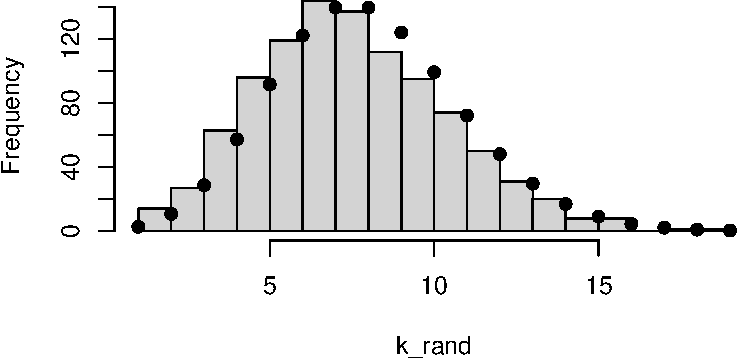
\includegraphics{./prob_files/figure-pdf/unnamed-chunk-12-2.pdf}

}

}

\end{minipage}%

\end{figure}

\hypertarget{footnotes-1}{%
\section{Footnotes}\label{footnotes-1}}

\hypertarget{sec-covariance}{%
\subsection{Covariance matrix}\label{sec-covariance}}

As reminder, the variance of a random variable, \(x\), with sample size
\(n\) is:
\[\sigma^2_x = \frac{1}{n-1} \sum_i^n (x_i - \bar{x})(x_i - \bar{x}) = \frac{1}{n-1} \sum_i^n (x_i - \bar{x})^2.\]
And \(\bar{x}\) is the sample mean. Similarly, then, the covariance of
samples from two random variables, \(x\) and \(y\), can be calculated
as:
\[\sigma(x,y) = \frac{1}{n-1} \sum_i^n (x_i - \bar{x})(y_i - \bar{y}).\]
The syntax for the covariance of a sample population with itself is, for
example, \(\sigma(x, x)\), which is simply equal to the variance
\(\sigma_x^2\). The covariance matrix for these two sample populations
would be: \[C = \begin{bmatrix}
\sigma(x,x) & \sigma(x,y)\\
\sigma(y,x) & \sigma(y,y)
\end{bmatrix}.\] This can be simplified using the variance notation:
\[C = \begin{bmatrix}
\sigma^2_x & \sigma(x,y)\\
\sigma(y,x) & \sigma^2_y
\end{bmatrix}.\]

\bookmarksetup{startatroot}

\hypertarget{sec-ols}{%
\chapter{Ordinary Least Squares}\label{sec-ols}}

\hypertarget{lecture-material-1}{%
\section{Lecture material}\label{lecture-material-1}}

Please download and print the lecture materials from
\href{https://bblearn.nau.edu/}{Bblearn} or the
\href{https://github.com/joseph-mihaljevic/inf511-book/tree/main/lecture-material}{GitHub
repo}. After lectures, the recordings will appear in the Bblearn
Collaborate Ultra section.

\hypertarget{in-class-code}{%
\section*{In-class Code}\label{in-class-code}}
\addcontentsline{toc}{section}{In-class Code}

\markright{In-class Code}

Remember that our goal is to estimate the linear relationship between
data observations of response variable, \(y\), and its measured
covariate, \(x\), following: \(Y = XB + \epsilon\), where
\(\epsilon \sim N(0, \sigma^2 I).\) Our coefficients to estimate are
therefore \(\hat{B}\), which is a column vector of the intercept and
slope. We also estimate the standard deviation of the residuals (i.e.,
residual error), \(\hat{\sigma}\). To estimate the coefficients, we are
attempting to minimize the residual sum of squares,
\(|| \epsilon || ^ 2\). See Footnotes~\ref{sec-crossprod} for more
information regarding this notation.

\hypertarget{generate-the-data}{%
\section{Generate the data}\label{generate-the-data}}

We'll start with a very small data set to emphasize the basics, and then
the in-class activity will go into more depth. Here, we'll implement the
OLS estimation with a single covariate that we demonstrated in lecture.

\begin{Shaded}
\begin{Highlighting}[]
\NormalTok{n }\OtherTok{=} \DecValTok{4} \CommentTok{\# number observations}
\NormalTok{p }\OtherTok{=} \DecValTok{2} \CommentTok{\# number of parameters}

\CommentTok{\# Covariate:}
\NormalTok{x0 }\OtherTok{=} \FunctionTok{c}\NormalTok{(}\DecValTok{1}\NormalTok{,}\DecValTok{1}\NormalTok{,}\DecValTok{1}\NormalTok{,}\DecValTok{1}\NormalTok{) }\CommentTok{\# placeholder for intercept}
\NormalTok{x1 }\OtherTok{=} \FunctionTok{c}\NormalTok{(}\DecValTok{2}\NormalTok{,}\DecValTok{3}\NormalTok{,}\DecValTok{5}\NormalTok{,}\DecValTok{1}\NormalTok{) }\CommentTok{\# value of x}
\NormalTok{xmat }\OtherTok{=} \FunctionTok{matrix}\NormalTok{(}\AttributeTok{data =} \FunctionTok{c}\NormalTok{(x0,x1), }
               \AttributeTok{nrow =}\NormalTok{ n, }
               \AttributeTok{ncol =}\NormalTok{ p)}
\NormalTok{xmat}
\end{Highlighting}
\end{Shaded}

\begin{verbatim}
     [,1] [,2]
[1,]    1    2
[2,]    1    3
[3,]    1    5
[4,]    1    1
\end{verbatim}

\begin{Shaded}
\begin{Highlighting}[]
\CommentTok{\# Coefficients:}
\DocumentationTok{\#\# betas[1]: intercept}
\DocumentationTok{\#\# betas[2]: slope}
\NormalTok{betas }\OtherTok{=} \FunctionTok{c}\NormalTok{(}\DecValTok{4}\NormalTok{, }\DecValTok{2}\NormalTok{)}

\NormalTok{xmat }\SpecialCharTok{\%*\%}\NormalTok{ betas}
\end{Highlighting}
\end{Shaded}

\begin{verbatim}
     [,1]
[1,]    8
[2,]   10
[3,]   14
[4,]    6
\end{verbatim}

\begin{Shaded}
\begin{Highlighting}[]
\CommentTok{\# residuals}
\NormalTok{epsilon }\OtherTok{=} \FunctionTok{c}\NormalTok{(}\DecValTok{0}\NormalTok{, }\SpecialCharTok{{-}}\DecValTok{1}\NormalTok{, }\DecValTok{1}\NormalTok{, }\DecValTok{3}\NormalTok{)}

\CommentTok{\# Data observations:}
\NormalTok{y }\OtherTok{=}\NormalTok{ xmat }\SpecialCharTok{\%*\%}\NormalTok{ betas }\SpecialCharTok{+}\NormalTok{ epsilon}
\end{Highlighting}
\end{Shaded}

\hypertarget{plot-the-relationship}{%
\section{Plot the relationship}\label{plot-the-relationship}}

\begin{Shaded}
\begin{Highlighting}[]
\CommentTok{\# Plot in layers}
\DocumentationTok{\#\# Create a blank plotting canvas, specifying axis limits}
\FunctionTok{plot}\NormalTok{(}\AttributeTok{x=}\ConstantTok{NA}\NormalTok{,}\AttributeTok{y=}\ConstantTok{NA}\NormalTok{, }\AttributeTok{xlab =} \StringTok{"x"}\NormalTok{, }\AttributeTok{ylab =} \StringTok{"y"}\NormalTok{,}
     \AttributeTok{ylim =} \FunctionTok{c}\NormalTok{(}\DecValTok{0}\NormalTok{,}\FunctionTok{max}\NormalTok{(y)), }\AttributeTok{xlim =} \FunctionTok{c}\NormalTok{(}\DecValTok{0}\NormalTok{,}\FunctionTok{max}\NormalTok{(x1)))}
\DocumentationTok{\#\# Add data points}
\FunctionTok{points}\NormalTok{(y }\SpecialCharTok{\textasciitilde{}}\NormalTok{ x1, }\AttributeTok{pch =} \DecValTok{19}\NormalTok{, }\AttributeTok{cex =} \DecValTok{2}\NormalTok{)}
\DocumentationTok{\#\# Add known linear relationship}
\FunctionTok{abline}\NormalTok{(}\AttributeTok{coef =}\NormalTok{ betas, }\AttributeTok{col =} \StringTok{"black"}\NormalTok{, }\AttributeTok{lwd =} \DecValTok{2}\NormalTok{)}

\CommentTok{\# Show the residuals:}
\FunctionTok{segments}\NormalTok{(}\AttributeTok{x0 =}\NormalTok{ x1, }\AttributeTok{x1 =}\NormalTok{ x1,}
         \AttributeTok{y0 =}\NormalTok{ y, }\AttributeTok{y1 =}\NormalTok{ y }\SpecialCharTok{{-}}\NormalTok{ epsilon)}

\CommentTok{\# Show the model predictions, \textbackslash{}hat\{y\}:}
\NormalTok{y\_hat }\OtherTok{=}\NormalTok{ xmat }\SpecialCharTok{\%*\%}\NormalTok{ betas}
\FunctionTok{points}\NormalTok{(y\_hat }\SpecialCharTok{\textasciitilde{}}\NormalTok{ x1, }\AttributeTok{cex =} \FloatTok{1.25}\NormalTok{)}
\end{Highlighting}
\end{Shaded}

\begin{figure}[H]

{\centering \includegraphics{./ols_files/figure-pdf/unnamed-chunk-4-1.pdf}

}

\end{figure}

\hypertarget{sec-lm-output}{%
\section{\texorpdfstring{Estimate the coefficients using R's
\texttt{lm()}
function}{Estimate the coefficients using R's lm() function}}\label{sec-lm-output}}

\begin{Shaded}
\begin{Highlighting}[]
\CommentTok{\# Run the model:}
\NormalTok{lm\_out }\OtherTok{=} \FunctionTok{lm}\NormalTok{(y }\SpecialCharTok{\textasciitilde{}} \DecValTok{1} \SpecialCharTok{+}\NormalTok{ x1)}
\CommentTok{\# Show the summary output}
\FunctionTok{summary}\NormalTok{(lm\_out)}
\end{Highlighting}
\end{Shaded}

\begin{verbatim}

Call:
lm(formula = y ~ 1 + x1)

Residuals:
     1      2      3      4 
-1.029 -1.657  1.086  1.600 

Coefficients:
            Estimate Std. Error t value Pr(>|t|)
(Intercept)   5.7714     2.0500   2.815    0.106
x1            1.6286     0.6565   2.481    0.131

Residual standard error: 1.942 on 2 degrees of freedom
Multiple R-squared:  0.7547,    Adjusted R-squared:  0.6321 
F-statistic: 6.153 on 1 and 2 DF,  p-value: 0.1313
\end{verbatim}

\begin{Shaded}
\begin{Highlighting}[]
\CommentTok{\# Extract the estimated coefficients}
\NormalTok{lm\_coef }\OtherTok{=} \FunctionTok{coef}\NormalTok{(lm\_out)}
\NormalTok{lm\_coef}
\end{Highlighting}
\end{Shaded}

\begin{verbatim}
(Intercept)          x1 
   5.771429    1.628571 
\end{verbatim}

\hypertarget{estimate-the-coefficients-manually}{%
\section{Estimate the coefficients
manually}\label{estimate-the-coefficients-manually}}

Now we will use the matrix algebra and derivation of normal equations to
estimate the intercept and slope from the observations, \(Y\). Remember
that we estimate the coefficient vector, \(\hat{B}\) from:
\[X^TX \hat{B} = X^T Y\] \[\hat{B} = (X^TX)^{-1} X^T Y\] These equations
include the multiplicative inverse matrix, \((X^TX)^{-1}\). See the
Footnotes~\ref{sec-solve} for more information about inverse matrices
and the \texttt{solve()} function.

\begin{Shaded}
\begin{Highlighting}[]
\CommentTok{\# Let\textquotesingle{}s break up the normal equations into intermediates:}
\NormalTok{xtx }\OtherTok{=} \FunctionTok{t}\NormalTok{(xmat) }\SpecialCharTok{\%*\%}\NormalTok{ xmat}

\DocumentationTok{\#\# Use solve() to find inverse of xtx}
\DocumentationTok{\#\# why solve()? See Appendix, linked above.}
\NormalTok{inv\_xtx }\OtherTok{=} \FunctionTok{solve}\NormalTok{(xtx)}
\NormalTok{xty }\OtherTok{=} \FunctionTok{t}\NormalTok{(xmat) }\SpecialCharTok{\%*\%}\NormalTok{ y}

\NormalTok{bhat }\OtherTok{=}\NormalTok{ inv\_xtx }\SpecialCharTok{\%*\%}\NormalTok{ xty}

\CommentTok{\# More efficient:}
\CommentTok{\# Remember, xtx * bhat = xty}
\CommentTok{\# So we can use solve() again}
\NormalTok{bhat\_solve }\OtherTok{=} \FunctionTok{solve}\NormalTok{(xtx, xty)}

\CommentTok{\# Are they the same?}

\CommentTok{\# How does this manual solution compare to lm()\textquotesingle{}s solution?}
\end{Highlighting}
\end{Shaded}

\hypertarget{sec-est-plot}{%
\section{\texorpdfstring{Plot the \emph{estimated}
relationships}{Plot the estimated relationships}}\label{sec-est-plot}}

\begin{Shaded}
\begin{Highlighting}[]
\CommentTok{\# Plot in layers}
\DocumentationTok{\#\# Create a blank plotting canvas, specifying axis limits}
\FunctionTok{plot}\NormalTok{(}\ConstantTok{NA}\NormalTok{,}\ConstantTok{NA}\NormalTok{,}
     \AttributeTok{xlab =} \StringTok{"x"}\NormalTok{, }\AttributeTok{ylab =} \StringTok{"y"}\NormalTok{,}
     \AttributeTok{ylim =} \FunctionTok{c}\NormalTok{(}\DecValTok{0}\NormalTok{,}\FunctionTok{max}\NormalTok{(y)),}
     \AttributeTok{xlim =} \FunctionTok{c}\NormalTok{(}\DecValTok{0}\NormalTok{,}\FunctionTok{max}\NormalTok{(x1)))}
\DocumentationTok{\#\# Add data points}
\FunctionTok{points}\NormalTok{(y }\SpecialCharTok{\textasciitilde{}}\NormalTok{ x1, }\AttributeTok{pch =} \DecValTok{19}\NormalTok{, }\AttributeTok{cex =} \DecValTok{2}\NormalTok{)}
\DocumentationTok{\#\# Add known linear relationship}
\FunctionTok{abline}\NormalTok{(}\AttributeTok{coef =}\NormalTok{ betas,}
       \AttributeTok{col =} \StringTok{"black"}\NormalTok{, }\AttributeTok{lwd =} \DecValTok{2}\NormalTok{)}

\CommentTok{\# Show the residuals:}
\FunctionTok{segments}\NormalTok{(}
  \AttributeTok{x0 =}\NormalTok{ x1,}
  \AttributeTok{x1 =}\NormalTok{ x1,}
  \AttributeTok{y0 =}\NormalTok{ y,}
  \AttributeTok{y1 =}\NormalTok{ y }\SpecialCharTok{{-}}\NormalTok{ epsilon,}
\NormalTok{)}

\CommentTok{\# Show the model predictions, \textbackslash{}hat\{y\}:}
\NormalTok{y\_hat }\OtherTok{=}\NormalTok{ xmat }\SpecialCharTok{\%*\%}\NormalTok{ betas}
\FunctionTok{points}\NormalTok{(y\_hat }\SpecialCharTok{\textasciitilde{}}\NormalTok{ x1,}
       \AttributeTok{cex =} \FloatTok{1.25}\NormalTok{)}

\CommentTok{\# Add the lm() estimate:}
\FunctionTok{abline}\NormalTok{(}\AttributeTok{coef =}\NormalTok{ lm\_coef,}
       \AttributeTok{col =} \StringTok{"orange"}\NormalTok{, }\AttributeTok{lty =} \DecValTok{2}\NormalTok{, }\AttributeTok{lwd =} \DecValTok{2}\NormalTok{)}

\CommentTok{\# Add the manual OLS estimate:}
\FunctionTok{abline}\NormalTok{(}\AttributeTok{coef =}\NormalTok{ bhat\_solve,}
       \AttributeTok{col =} \StringTok{"purple"}\NormalTok{, }\AttributeTok{lty =} \DecValTok{3}\NormalTok{, }\AttributeTok{lwd =} \DecValTok{2}\NormalTok{)}
\end{Highlighting}
\end{Shaded}

\begin{figure}[H]

{\centering \includegraphics{./ols_files/figure-pdf/unnamed-chunk-10-1.pdf}

}

\end{figure}

\hypertarget{why-are-the-hatb-different-from-true-b}{%
\section{\texorpdfstring{Why are the \(\hat{B}\) different from true
\(B\)?}{Why are the \textbackslash hat\{B\} different from true B?}}\label{why-are-the-hatb-different-from-true-b}}

Remember, we are estimating the coefficients by minimizing the sum of
squared errors (SSE), \(|| \epsilon ||^2\).

\begin{Shaded}
\begin{Highlighting}[]
\CommentTok{\# True sum of squares:}
\FunctionTok{sum}\NormalTok{(epsilon)}\SpecialCharTok{\^{}}\DecValTok{2}
\end{Highlighting}
\end{Shaded}

\begin{verbatim}
[1] 9
\end{verbatim}

\begin{Shaded}
\begin{Highlighting}[]
\CommentTok{\# Estimated (i.e., minimized sum of squares):}
\DocumentationTok{\#\# From lm()}
\FunctionTok{sum}\NormalTok{(lm\_out}\SpecialCharTok{$}\NormalTok{residuals)}\SpecialCharTok{\^{}}\DecValTok{2}
\end{Highlighting}
\end{Shaded}

\begin{verbatim}
[1] 0
\end{verbatim}

\begin{Shaded}
\begin{Highlighting}[]
\DocumentationTok{\#\# From manual OLS}
\FunctionTok{sum}\NormalTok{( (y }\SpecialCharTok{{-}}\NormalTok{ xmat }\SpecialCharTok{\%*\%}\NormalTok{ bhat\_solve) )}\SpecialCharTok{\^{}}\DecValTok{2}
\end{Highlighting}
\end{Shaded}

\begin{verbatim}
[1] 7.099748e-30
\end{verbatim}

You can see that the OLS strategy effectively minimized the SSE to zero.

\hypertarget{understanding-uncertainty-in-hatb}{%
\section{\texorpdfstring{Understanding Uncertainty in
\(\hat{B}\)}{Understanding Uncertainty in \textbackslash hat\{B\}}}\label{understanding-uncertainty-in-hatb}}

While the OLS analysis estimates the regression coefficients,
\(\hat{B}\), from the observed data \(Y\), our estimates of these
coefficients have error (i.e., uncertainty), such that the estimates are
only as good as the data. Specifically, if we have fewer data points
(i.e., \(n\) is low), we have less certainty in \(\hat{B}\). In lecture,
we showed, that:
\[\hat{B} \sim N \left( B, (X^TX)^{-1} \hat{\sigma}^2 \right), \] and we
know that \(\hat{\sigma}^2\) depends on sample size \(n\), following:
\[\hat{\sigma}^2 \quad = \quad \frac{1}{n-p} (Y_{obs} - Y_{pred})^T (Y_{obs} - Y_{pred}) \quad = \quad \frac{1}{n-p} \hat{\epsilon}^T \hat{\epsilon}\]

Using these equations, we showed then that
\(SE(\beta_i) = \sqrt{diag\left( (X^TX)^{-1} \right)_i \hat{\sigma}^2}\).
Let's calculate this manually and compare to the output of the
\texttt{lm()} function.

\begin{Shaded}
\begin{Highlighting}[]
\CommentTok{\# Extract the model summary, which has useful components}
\NormalTok{lm\_out\_summary }\OtherTok{=} \FunctionTok{summary}\NormalTok{(lm\_out)}
\CommentTok{\# Extract the estimated residual standard deviation, sigma}
\NormalTok{est\_sigma }\OtherTok{=}\NormalTok{ lm\_out\_summary}\SpecialCharTok{$}\NormalTok{sigma}
\NormalTok{est\_sigma}
\end{Highlighting}
\end{Shaded}

\begin{verbatim}
[1] 1.942017
\end{verbatim}

\begin{Shaded}
\begin{Highlighting}[]
\CommentTok{\# We already calculated (X\^{}T X)\^{}\{{-}1\} as inv\_xtx}
\NormalTok{beta\_cov\_mat }\OtherTok{=}\NormalTok{ inv\_xtx }\SpecialCharTok{*}\NormalTok{ est\_sigma}\SpecialCharTok{\^{}}\DecValTok{2}
\NormalTok{beta\_cov\_mat}
\end{Highlighting}
\end{Shaded}

\begin{verbatim}
          [,1]       [,2]
[1,]  4.202449 -1.1853061
[2,] -1.185306  0.4310204
\end{verbatim}

\begin{Shaded}
\begin{Highlighting}[]
\NormalTok{se\_beta }\OtherTok{=} \FunctionTok{sqrt}\NormalTok{(}\FunctionTok{diag}\NormalTok{(beta\_cov\_mat))}
\NormalTok{se\_beta}
\end{Highlighting}
\end{Shaded}

\begin{verbatim}
[1] 2.0499876 0.6565214
\end{verbatim}

Compare these values to the output of the \texttt{summary()} of
Section~\ref{sec-lm-output} in the column labelled \texttt{Std.\ Error}.

\hypertarget{sec-conf-beta}{%
\section{\texorpdfstring{Confidence Intervals for
\(\hat{B}\)}{Confidence Intervals for \textbackslash hat\{B\}}}\label{sec-conf-beta}}

To calculate confidence intervals for \(\hat{B}\), we first must
understand the \(t\) (a.k.a. Student's \(t\)) probability distribution.
This distribution represents the case when we are estimating the mean of
a normally distributed variable and either the sample size is small or
the variable's standard deviation is unknown. Essentially, the \(t\)
distribution increases the uncertainty (i.e., variance) in cases of low
sample size (i.e., small \(n\)). With low sample size (and/or high
number of parameters), the degrees of freedom of the \(t\)-distribution,
\(\nu\) is low, whereas with high sample size, \(\nu\) is large. As
\(\nu\) approaches infinity, the \(t\)-distribution approximates the
standard normal distribution (i.e., \(N(\mu, \sigma)|\mu=0,\sigma=1\)).

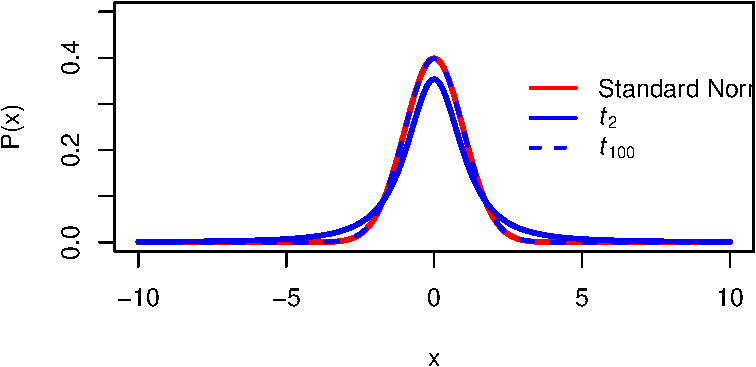
\includegraphics{./ols_files/figure-pdf/unnamed-chunk-16-1.pdf}

It is the case for
\(\hat{B} \sim N \left( B, (X^TX)^{-1} \hat{\sigma}^2 \right)\) that we
do not know the mean (\(B\)), and we are estimating the variance,
\(\hat{\sigma}^2\). Specifically, we are estimating the true mean
vector, \(B\), as \(\hat{B}\), and we are estimating the variance of the
residuals as \(\hat{\sigma}^2\). We can therefore re-write the
uncertainty in \(\hat{B}\) as a multivariate \(t\) distribution:
\[(\hat{B} - B) \sim t_{\nu} \left( 0, \Sigma \right),\] where the means
are zero, \(\nu\) is the degrees of freedom (i.e., \(n-p\)), and
\(\Sigma = (X^TX)^{-1} \hat{\sigma}^2\). \((\hat{B} - B)\) represents
the deviation of the estimated coefficients from the true coefficients,
which is why the distribution is centered around zero. It is perhaps
easier to separate the individual estimated coefficients, \(\beta_i\),
into their separate \(t\)-distributions:
\[\frac{(\hat{\beta}_i - \beta_i)}{SE(\hat{\beta}_i)} \sim t_{\nu}\]
\[(\hat{\beta}_i - \beta_i) \sim t_{\nu} SE(\hat{\beta}_i),\] which
shows that the \(t\)-distribution that describes the deviation of
regression coefficients from the true value of those coefficients is
scaled by the uncertainty in the estimated coefficients
\(SE(\hat{\beta}_i)\). As shown in Dr.~Barber's materials, using this
information, we can derive the confidence interval (at the \(\alpha\)
confidence level) calculation for \(\hat{\beta}_i\) as:
\[ \hat{\beta}_i \pm t \left(\frac{1-\alpha}{2}, \nu \right) SE(\hat{\beta}_i),\]
where the \(t()\) notation represents the \emph{critical value} of the
\(t\)-distribution, \(t_{crit}\), with \(\nu\) degrees of freedom, for
which \(P(z \le t_{crit}) = \frac{1-\alpha}{2}\), and \(z\) is a
continuous, random variable. This critical value can be calculated in R
using the \texttt{qt()} function, which we show below.

\begin{tcolorbox}[enhanced jigsaw, colback=white, title=\textcolor{quarto-callout-note-color}{\faInfo}\hspace{0.5em}{Covariance of \(\hat{\beta}_i\)}, left=2mm, coltitle=black, bottomrule=.15mm, arc=.35mm, toprule=.15mm, rightrule=.15mm, opacityback=0, opacitybacktitle=0.6, colframe=quarto-callout-note-color-frame, leftrule=.75mm, toptitle=1mm, titlerule=0mm, breakable, bottomtitle=1mm, colbacktitle=quarto-callout-note-color!10!white]

Although it is convenient and easier to digest the confidence interval
of individual \(\hat{\beta}_i\), we must realize that the estimates of
the \(\beta_i\) can covary (i.e., have non-zero covariance), which is
quantified in the variance-covariance matrix of \(\hat{B}\),
\((X^TX)^{-1} \hat{\sigma}^2\). We will show why this is important
below.

\end{tcolorbox}

Let's manually calculate the 95\% confidence intervals in \(\hat{B}\)
and compare to R's internal function \texttt{confint()}.

\begin{Shaded}
\begin{Highlighting}[]
\CommentTok{\# Extract the degrees of freedom from the model (\textbackslash{}nu)}
\CommentTok{\# which can also be calculated as n {-} p}
\NormalTok{t\_df }\OtherTok{=}\NormalTok{ lm\_out}\SpecialCharTok{$}\NormalTok{df.residual}

\CommentTok{\# Calculate t critical for alpha = 0.05}
\CommentTok{\# This will give us the 95\% conf interval (CI)}
\NormalTok{t\_crit }\OtherTok{=} \FunctionTok{qt}\NormalTok{(}\DecValTok{1}\SpecialCharTok{{-}}\NormalTok{(}\FloatTok{0.05}\SpecialCharTok{/}\DecValTok{2}\NormalTok{), }\AttributeTok{df =}\NormalTok{ t\_df)}

\CommentTok{\# Calculate the upper and lower CI for both betas}
\NormalTok{ci\_int }\OtherTok{=}\NormalTok{ lm\_coef[}\DecValTok{1}\NormalTok{] }\SpecialCharTok{+} \FunctionTok{c}\NormalTok{(}\SpecialCharTok{{-}}\DecValTok{1}\NormalTok{,}\DecValTok{1}\NormalTok{)}\SpecialCharTok{*}\NormalTok{t\_crit}\SpecialCharTok{*}\NormalTok{se\_beta[}\DecValTok{1}\NormalTok{]}
\NormalTok{ci\_slope }\OtherTok{=}\NormalTok{ lm\_coef[}\DecValTok{2}\NormalTok{] }\SpecialCharTok{+} \FunctionTok{c}\NormalTok{(}\SpecialCharTok{{-}}\DecValTok{1}\NormalTok{,}\DecValTok{1}\NormalTok{)}\SpecialCharTok{*}\NormalTok{t\_crit}\SpecialCharTok{*}\NormalTok{se\_beta[}\DecValTok{2}\NormalTok{]}

\CommentTok{\# Construct a table of values}
\NormalTok{ci\_mat }\OtherTok{=} 
    \FunctionTok{rbind}\NormalTok{(}\FunctionTok{c}\NormalTok{(lm\_coef[}\DecValTok{1}\NormalTok{], ci\_int),}
          \FunctionTok{c}\NormalTok{(lm\_coef[}\DecValTok{2}\NormalTok{], ci\_slope))}
\FunctionTok{colnames}\NormalTok{(ci\_mat) }\OtherTok{=} \FunctionTok{c}\NormalTok{(}\StringTok{"coef"}\NormalTok{, }\StringTok{"lowCI"}\NormalTok{, }\StringTok{"highCI"}\NormalTok{)}
\FunctionTok{rownames}\NormalTok{(ci\_mat) }\OtherTok{=} \FunctionTok{c}\NormalTok{(}\StringTok{"intercept"}\NormalTok{, }\StringTok{"slope"}\NormalTok{)}
\NormalTok{ci\_mat}
\end{Highlighting}
\end{Shaded}

\begin{verbatim}
              coef     lowCI    highCI
intercept 5.771429 -3.048956 14.591813
slope     1.628571 -1.196212  4.453355
\end{verbatim}

\begin{Shaded}
\begin{Highlighting}[]
\CommentTok{\# Compare these manual calculations to built{-}in}
\CommentTok{\# function confint(), which by default extracts the }
\CommentTok{\# 95\% CI for a lm() model\textquotesingle{}s coefficients}
\FunctionTok{confint}\NormalTok{(lm\_out)}
\end{Highlighting}
\end{Shaded}

\begin{verbatim}
                2.5 %    97.5 %
(Intercept) -3.048956 14.591813
x1          -1.196212  4.453355
\end{verbatim}

\hypertarget{propagate-uncertainty-in-hatb-for-predictions-of-y}{%
\section{\texorpdfstring{Propagate uncertainty in \(\hat{B}\) for
predictions of
\(Y\)}{Propagate uncertainty in \textbackslash hat\{B\} for predictions of Y}}\label{propagate-uncertainty-in-hatb-for-predictions-of-y}}

There are several ways to calculate and visualize our uncertainty in
model predictions of observed data \(Y\) and unobserved data of the
dependent variable (i.e., interpolation). The colored lines drawn on the
figure in Section~\ref{sec-est-plot} represent the expected values of
\(Y\) based on the OLS analysis' estimate of \(\hat{B}\), but this line
does not include uncertainty in these coefficient values.

\hypertarget{multivariate-t-distribution-method}{%
\subsection{\texorpdfstring{Multivariate \(t\)-distribution
method}{Multivariate t-distribution method}}\label{multivariate-t-distribution-method}}

First, we will calculate uncertainty by sampling from the multivariate
\(t\) distribution that represents error in regression coefficients,
\(\hat{B}\).

\begin{Shaded}
\begin{Highlighting}[]
\CommentTok{\# We will "bootstrap" 1000 samples of intercept and slope}
\FunctionTok{set.seed}\NormalTok{(}\DecValTok{3}\NormalTok{)}
\NormalTok{n\_samp }\OtherTok{=} \DecValTok{500}

\CommentTok{\# Draw from the multivariate t }
\CommentTok{\# which represents (\textbackslash{}hat\{B\} {-} B)}
\NormalTok{test\_mat\_deviates }\OtherTok{=} 
\NormalTok{  mnormt}\SpecialCharTok{::}\FunctionTok{rmt}\NormalTok{(n\_samp, }\AttributeTok{mean =} \FunctionTok{c}\NormalTok{(}\DecValTok{0}\NormalTok{,}\DecValTok{0}\NormalTok{), }\AttributeTok{S =}\NormalTok{ beta\_cov\_mat, }\AttributeTok{df =}\NormalTok{ t\_df)}

\CommentTok{\# Now calculate the realized intercept and slope}
\CommentTok{\# using the t{-}distributed deviates}
\NormalTok{test\_mat\_t }\OtherTok{=} \FunctionTok{cbind}\NormalTok{(}
\NormalTok{  lm\_coef[}\DecValTok{1}\NormalTok{] }\SpecialCharTok{+} \FunctionTok{c}\NormalTok{(test\_mat\_deviates[,}\DecValTok{1}\NormalTok{]),}
\NormalTok{  lm\_coef[}\DecValTok{2}\NormalTok{] }\SpecialCharTok{+} \FunctionTok{c}\NormalTok{(test\_mat\_deviates[,}\DecValTok{2}\NormalTok{])}
\NormalTok{)}

\CommentTok{\# Calculate the 95\% quantiles and compare to the }
\CommentTok{\# calculated 95\% confidence intervals from above}
\FunctionTok{apply}\NormalTok{(test\_mat\_t, }
      \AttributeTok{MARGIN =} \DecValTok{2}\NormalTok{, }\CommentTok{\# applies function (FUN) to columns (dim 2)}
      \AttributeTok{FUN =}\NormalTok{ quantile, }\AttributeTok{probs =} \FunctionTok{c}\NormalTok{(}\FloatTok{0.025}\NormalTok{, }\FloatTok{0.5}\NormalTok{, }\FloatTok{0.975}\NormalTok{))}
\end{Highlighting}
\end{Shaded}

\begin{verbatim}
           [,1]       [,2]
2.5%  -3.820226 -0.5319227
50%    5.809501  1.5967318
97.5% 13.564890  4.1240734
\end{verbatim}

\begin{Shaded}
\begin{Highlighting}[]
\CommentTok{\# Compare}
\NormalTok{ci\_mat}
\end{Highlighting}
\end{Shaded}

\begin{verbatim}
              coef     lowCI    highCI
intercept 5.771429 -3.048956 14.591813
slope     1.628571 -1.196212  4.453355
\end{verbatim}

\begin{Shaded}
\begin{Highlighting}[]
\CommentTok{\# Plot the relationship between intercept and slope}
\CommentTok{\# Notice the covariance}
\FunctionTok{plot}\NormalTok{(test\_mat\_t, }\AttributeTok{xlab =} \StringTok{"Intercept"}\NormalTok{, }\AttributeTok{ylab =} \StringTok{"Slope"}\NormalTok{)}
\end{Highlighting}
\end{Shaded}

\begin{figure}[H]

{\centering \includegraphics{./ols_files/figure-pdf/unnamed-chunk-20-1.pdf}

}

\end{figure}

Next, for each pair of intercept and slope randomly drawn above, we will
calculate the expected values of \(Y\) across the range of covariate
\(x\). We will then summarize the 95\% quantile of expected \(Y\) at
each value of \(x\) in this interpolation. To do this, we need a
function to calculate the expected value of \(Y\). This function will
have the intercept and slope as inputs and will output the expected
values of \(Y\) across a range of \(x\). Then, we will \texttt{apply()}
this function using all of the values of intercept and slope, in a
vectorized and therefore very efficient manner, rather than using any
\texttt{for} loops.

\begin{Shaded}
\begin{Highlighting}[]
\CommentTok{\# Create a matrix that holds the values of x}
\CommentTok{\# over which we want to interpolate the expected}
\CommentTok{\# values of Y}
\NormalTok{x\_fake\_mat }\OtherTok{=} 
  \FunctionTok{cbind}\NormalTok{(}
    \FunctionTok{rep}\NormalTok{(}\DecValTok{1}\NormalTok{, }\AttributeTok{times =} \DecValTok{100}\NormalTok{),}
    \FunctionTok{seq}\NormalTok{(}\DecValTok{0}\NormalTok{,}\FunctionTok{max}\NormalTok{(x1),}\AttributeTok{length.out =} \DecValTok{100}\NormalTok{)}
\NormalTok{  )}

\CommentTok{\# Create a function that will calculate the expected values}
\NormalTok{y\_hat\_fun }\OtherTok{=} \ControlFlowTok{function}\NormalTok{(x, x\_mat)\{}
\NormalTok{  x\_mat }\SpecialCharTok{\%*\%}\NormalTok{ x}
\NormalTok{\}}

\CommentTok{\# Apply this function to all intercepts and slopes that}
\CommentTok{\# we drew from the multivariate t}
\NormalTok{y\_pred\_mt }\OtherTok{=} \FunctionTok{apply}\NormalTok{(test\_mat\_t, }\DecValTok{1}\NormalTok{, y\_hat\_fun, }\AttributeTok{x\_mat=}\NormalTok{x\_fake\_mat)}

\CommentTok{\# Summarize the 95\% quantile of the expected value of Y}
\CommentTok{\# at each value of x }
\NormalTok{y\_pred\_mt\_summary }\OtherTok{=} \FunctionTok{apply}\NormalTok{(y\_pred\_mt, }\DecValTok{1}\NormalTok{, quantile, }\AttributeTok{probs =} \FunctionTok{c}\NormalTok{(}\FloatTok{0.025}\NormalTok{, }\FloatTok{0.975}\NormalTok{))}
\FunctionTok{str}\NormalTok{(y\_pred\_mt\_summary)}
\end{Highlighting}
\end{Shaded}

\begin{verbatim}
 num [1:2, 1:100] -3.82 13.56 -3.62 13.58 -3.41 ...
 - attr(*, "dimnames")=List of 2
  ..$ : chr [1:2] "2.5%" "97.5%"
  ..$ : NULL
\end{verbatim}

\hypertarget{predict-function-method}{%
\subsection{\texorpdfstring{\texttt{predict()} function
method}{predict() function method}}\label{predict-function-method}}

R has a built-in function \texttt{predict()} (see specific variant
\texttt{predict.lm()}) which calculates expected values of the dependent
variable from a linear regression model estimated using the function
\texttt{lm()}.

\begin{Shaded}
\begin{Highlighting}[]
\CommentTok{\# Note that \textquotesingle{}newdata\textquotesingle{} must be a data frame that includes the ranges}
\CommentTok{\# of each covariate in the regression model for which you want }
\CommentTok{\# to generate interpolated or predicted values of the dependent variable}

\CommentTok{\# Here we are calculated the expected values as well as the }
\CommentTok{\# 95\% confidence intervals for those expected values}
\NormalTok{y\_predict }\OtherTok{=} \FunctionTok{predict}\NormalTok{(lm\_out,}
                 \AttributeTok{newdata =} \FunctionTok{data.frame}\NormalTok{(}\AttributeTok{x1 =} \FunctionTok{c}\NormalTok{(x\_fake\_mat[,}\DecValTok{2}\NormalTok{])),}
                 \AttributeTok{interval =} \StringTok{"confidence"}\NormalTok{, }\AttributeTok{level =} \FloatTok{0.95}\NormalTok{)}
\FunctionTok{str}\NormalTok{(y\_predict)}
\end{Highlighting}
\end{Shaded}

\begin{verbatim}
 num [1:100, 1:3] 5.77 5.85 5.94 6.02 6.1 ...
 - attr(*, "dimnames")=List of 2
  ..$ : chr [1:100] "1" "2" "3" "4" ...
  ..$ : chr [1:3] "fit" "lwr" "upr"
\end{verbatim}

\hypertarget{compare-the-two-methods}{%
\subsection{Compare the two methods}\label{compare-the-two-methods}}

Let's visualize the output of the two methods to compare.

\begin{Shaded}
\begin{Highlighting}[]
\CommentTok{\# plot}
\FunctionTok{plot}\NormalTok{(}\AttributeTok{x=}\ConstantTok{NA}\NormalTok{,}\AttributeTok{y=}\ConstantTok{NA}\NormalTok{,}\AttributeTok{xlab =} \StringTok{"x"}\NormalTok{, }\AttributeTok{ylab =} \StringTok{"y"}\NormalTok{,}
     \AttributeTok{xlim =} \FunctionTok{c}\NormalTok{(}\DecValTok{0}\NormalTok{,}\FunctionTok{max}\NormalTok{(x1)), }\AttributeTok{ylim =} \FunctionTok{c}\NormalTok{(}\SpecialCharTok{{-}}\DecValTok{5}\NormalTok{, }\DecValTok{25}\NormalTok{), }\AttributeTok{pch =} \DecValTok{19}\NormalTok{)}
\CommentTok{\# Plot the expected values of Y for each pair of int/slope }
\ControlFlowTok{for}\NormalTok{(i }\ControlFlowTok{in} \DecValTok{1}\SpecialCharTok{:}\NormalTok{n\_samp)\{}
  \FunctionTok{lines}\NormalTok{(y\_pred\_mt[,i] }\SpecialCharTok{\textasciitilde{}}\NormalTok{ x\_fake\_mat[,}\DecValTok{2}\NormalTok{],}
        \CommentTok{\# Reduce the opacity of each line}
        \AttributeTok{col =}\NormalTok{ scales}\SpecialCharTok{::}\FunctionTok{alpha}\NormalTok{(}\StringTok{"black"}\NormalTok{, }\AttributeTok{alpha =} \FloatTok{0.1}\NormalTok{), }\AttributeTok{lwd =} \DecValTok{2}\NormalTok{)}
\NormalTok{\}}
\CommentTok{\# Add the data points}
\FunctionTok{points}\NormalTok{(y }\SpecialCharTok{\textasciitilde{}}\NormalTok{ x1, }\AttributeTok{col =} \StringTok{\textquotesingle{}orange\textquotesingle{}}\NormalTok{, }\AttributeTok{pch =} \DecValTok{19}\NormalTok{, }\AttributeTok{cex =} \DecValTok{2}\NormalTok{)}
\CommentTok{\# Add the expected values of Y from \textbackslash{}hat\{B\}}
\FunctionTok{abline}\NormalTok{(}\AttributeTok{coef =}\NormalTok{ lm\_coef, }\AttributeTok{col =} \StringTok{"orange"}\NormalTok{, }\AttributeTok{lwd =} \DecValTok{3}\NormalTok{)}
\CommentTok{\# Add the conf int of expected Y using multivariate t}
\FunctionTok{lines}\NormalTok{(y\_pred\_mt\_summary[}\DecValTok{1}\NormalTok{,] }\SpecialCharTok{\textasciitilde{}}\NormalTok{ x\_fake\_mat[,}\DecValTok{2}\NormalTok{], }\AttributeTok{lty =} \DecValTok{2}\NormalTok{, }\AttributeTok{lwd =} \DecValTok{3}\NormalTok{, }\AttributeTok{col =} \StringTok{"orange"}\NormalTok{)}
\FunctionTok{lines}\NormalTok{(y\_pred\_mt\_summary[}\DecValTok{2}\NormalTok{,] }\SpecialCharTok{\textasciitilde{}}\NormalTok{ x\_fake\_mat[,}\DecValTok{2}\NormalTok{], }\AttributeTok{lty =} \DecValTok{2}\NormalTok{, }\AttributeTok{lwd =} \DecValTok{3}\NormalTok{, }\AttributeTok{col =} \StringTok{"orange"}\NormalTok{)}
\CommentTok{\# Add the conf int of expected Y using predict() function}
\FunctionTok{lines}\NormalTok{(y\_predict[,}\StringTok{"lwr"}\NormalTok{]}\SpecialCharTok{\textasciitilde{}}\NormalTok{ x\_fake\_mat[,}\DecValTok{2}\NormalTok{], }\AttributeTok{lty =} \DecValTok{3}\NormalTok{, }\AttributeTok{lwd =} \DecValTok{3}\NormalTok{, }\AttributeTok{col =} \StringTok{"purple"}\NormalTok{)}
\FunctionTok{lines}\NormalTok{(y\_predict[,}\StringTok{"upr"}\NormalTok{]}\SpecialCharTok{\textasciitilde{}}\NormalTok{ x\_fake\_mat[,}\DecValTok{2}\NormalTok{], }\AttributeTok{lty =} \DecValTok{3}\NormalTok{, }\AttributeTok{lwd =} \DecValTok{3}\NormalTok{, }\AttributeTok{col =} \StringTok{"purple"}\NormalTok{)}
\end{Highlighting}
\end{Shaded}

\begin{figure}[H]

{\centering 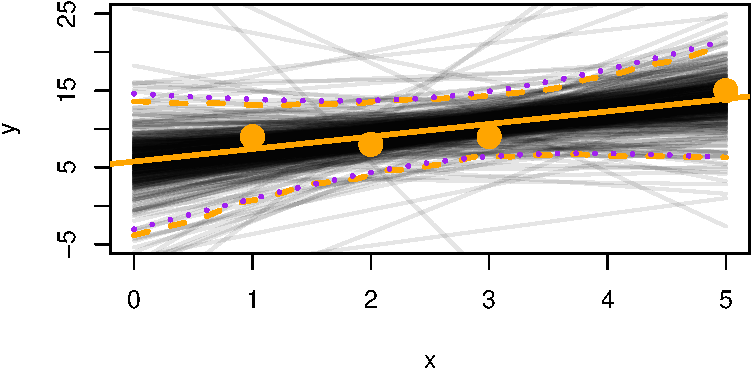
\includegraphics{./ols_files/figure-pdf/unnamed-chunk-26-1.pdf}

}

\end{figure}

There is yet a third option to calculate the uncertainty in predicted
(i.e., interpolated or extrapolated) values of \(Y\), which is to derive
an exact calculation of the confidence interval using the \(t\)
distribution, similar to that shown in Section~\ref{sec-conf-beta}. See
Ch4.1 of Dr.~Barber's book for this derivation.

\hypertarget{footnotes-2}{%
\section{Footnotes}\label{footnotes-2}}

\hypertarget{sec-crossprod}{%
\subsection{Euclidean norm \& cross product}\label{sec-crossprod}}

We often see the syntax, \(|| a ||\), which is the Euclidean norm of the
\(n\)-sized vector \(a\):
\[|| a || = \left( \sum_{i=1}^{n} a_i^2 \right) ^ {1/2} ,\] so that when
we see \(|| a ||^2\), this results in the sum of squares of vector
\(a\), \(\sum_{i=1}^{n} a_i^2\).

In the context of least squares regression, we are trying to minimize
the residual sum of squares, where the residuals, \(\epsilon_i\), are in
vector, \(\epsilon\). The sum of squares of vector \(\epsilon\) is
therefore \(|| \epsilon ||^2\). Algebraically, we can find this value as
the cross product of \(\epsilon\), which is \(\epsilon^{T}\epsilon\).
Let's do a coded example with vector \(x\).

\begin{Shaded}
\begin{Highlighting}[]
\CommentTok{\# Vector of real numbers}
\NormalTok{x }\OtherTok{=} \FunctionTok{c}\NormalTok{(}\DecValTok{1}\NormalTok{, }\DecValTok{2}\NormalTok{, }\DecValTok{3}\NormalTok{, }\DecValTok{4}\NormalTok{)}

\CommentTok{\# sum of squares}
\FunctionTok{sum}\NormalTok{(x}\SpecialCharTok{\^{}}\DecValTok{2}\NormalTok{)}
\end{Highlighting}
\end{Shaded}

\begin{verbatim}
[1] 30
\end{verbatim}

\begin{Shaded}
\begin{Highlighting}[]
\CommentTok{\# Evaluated as cross{-}product}
\FunctionTok{t}\NormalTok{(x) }\SpecialCharTok{\%*\%}\NormalTok{ x}
\end{Highlighting}
\end{Shaded}

\begin{verbatim}
     [,1]
[1,]   30
\end{verbatim}

\begin{Shaded}
\begin{Highlighting}[]
\DocumentationTok{\#\# Or with crossprod()}
\FunctionTok{crossprod}\NormalTok{(x,x)}
\end{Highlighting}
\end{Shaded}

\begin{verbatim}
     [,1]
[1,]   30
\end{verbatim}

\begin{Shaded}
\begin{Highlighting}[]
\CommentTok{\# Euclidean norm also known as the 2{-}norm}
\CommentTok{\# so sum of squares is 2{-}norm, squared}
\FunctionTok{norm}\NormalTok{(x, }\AttributeTok{type =} \StringTok{"2"}\NormalTok{) }\SpecialCharTok{\^{}} \DecValTok{2}
\end{Highlighting}
\end{Shaded}

\begin{verbatim}
[1] 30
\end{verbatim}

\hypertarget{sec-solve}{%
\subsection{\texorpdfstring{\texttt{solve()} and Inverse of
matrix}{solve() and Inverse of matrix}}\label{sec-solve}}

Suppose we have matrices \(A\), \(X\), and \(B\), and the following
expression is true: \[AX=B.\]

Then, suppose \(X\) is unknown, such that we want to find the solution
for \(X\), when we rearrange: \[X = A^{-1} B,\] where \(A^{-1}\) is the
multiplicative inverse of matrix \(A\). To figure this out
computationally, we can use the \texttt{solve()} function in R, as long
as \(A\) is a square matrix and has an inverse.

\begin{Shaded}
\begin{Highlighting}[]
\CommentTok{\# Create A and known X}
\NormalTok{A }\OtherTok{=} \FunctionTok{matrix}\NormalTok{(}\FunctionTok{c}\NormalTok{(}\DecValTok{1}\NormalTok{,}\DecValTok{1}\NormalTok{,}
             \DecValTok{5}\NormalTok{,}\DecValTok{2}\NormalTok{), }\AttributeTok{ncol =} \DecValTok{2}\NormalTok{)}
\NormalTok{X }\OtherTok{=} \FunctionTok{matrix}\NormalTok{(}\FunctionTok{c}\NormalTok{(}\DecValTok{2}\NormalTok{,}\DecValTok{3}\NormalTok{), }\AttributeTok{ncol =} \DecValTok{1}\NormalTok{)}

\CommentTok{\# Dot product to calculate B}
\NormalTok{B }\OtherTok{=}\NormalTok{ A }\SpecialCharTok{\%*\%}\NormalTok{ X}

\CommentTok{\# Suppose you have A and B, but want to find X}
\NormalTok{X\_solve }\OtherTok{=} \FunctionTok{solve}\NormalTok{(A, B)}

\CommentTok{\# Did it work?}
\NormalTok{X; X\_solve}
\end{Highlighting}
\end{Shaded}

\begin{verbatim}
     [,1]
[1,]    2
[2,]    3
\end{verbatim}

\begin{verbatim}
     [,1]
[1,]    2
[2,]    3
\end{verbatim}

We can see, then, that \texttt{solve()} is internally evaluating
\(A^{-1}\). Remember that \(A^{-1}\) is not trivial to calculate, as it
is the matrix that must satisfy: \(AA^{-1} = I\), where \(I\) is an
identity matrix. In fact, \texttt{solve(A)} returns the inverse of
\(A\), if it exists.

\begin{Shaded}
\begin{Highlighting}[]
\NormalTok{inv\_A }\OtherTok{=} \FunctionTok{solve}\NormalTok{(A)}

\CommentTok{\#Did it work?}
\NormalTok{(inv\_A }\SpecialCharTok{\%*\%}\NormalTok{ B)}
\end{Highlighting}
\end{Shaded}

\begin{verbatim}
     [,1]
[1,]    2
[2,]    3
\end{verbatim}

\begin{Shaded}
\begin{Highlighting}[]
\NormalTok{X}
\end{Highlighting}
\end{Shaded}

\begin{verbatim}
     [,1]
[1,]    2
[2,]    3
\end{verbatim}

\bookmarksetup{startatroot}

\hypertarget{sec-hypothesis}{%
\chapter{Hypothesis Testing}\label{sec-hypothesis}}

TBA

\bookmarksetup{startatroot}

\hypertarget{sec-max-lik}{%
\chapter{Maximum Likelihood}\label{sec-max-lik}}

TBA

\bookmarksetup{startatroot}

\hypertarget{sec-anova}{%
\chapter{ANOVA}\label{sec-anova}}

TBA

\bookmarksetup{startatroot}

\hypertarget{sec-bayesian}{%
\chapter{Bayesian inference}\label{sec-bayesian}}

TBA

\bookmarksetup{startatroot}

\hypertarget{references}{%
\chapter*{References}\label{references}}
\addcontentsline{toc}{chapter}{References}

\markboth{References}{References}

\hypertarget{refs}{}
\begin{CSLReferences}{1}{0}
\leavevmode\vadjust pre{\hypertarget{ref-knuth84}{}}%
Knuth, Donald E. 1984. {``Literate Programming.''} \emph{Comput. J.} 27
(2): 97--111. \url{https://doi.org/10.1093/comjnl/27.2.97}.

\end{CSLReferences}

\appendix
\addcontentsline{toc}{part}{Appendices}

\hypertarget{sec-syllabus}{%
\chapter{Syllabus}\label{sec-syllabus}}

\begin{figure}

{\centering 
\includegraphics{./images/nau_siccs_logo.png}

}

\end{figure}

\begin{itemize}
\tightlist
\item
  INF 511 Modern Regression I Spring 2023
\item
  3 units
\item
  Section 001: MW 4:00-5:15p, Science \& Health, Room 211
\item
  Section 002: MW 12:45-2:00p, Engineering, Room 120
\item
  Prerequisite: Admission to SICCS graduate program, STA 270, and ((MAT
  136 and MAT 137) or MAT 131))
\item
  Mode of Instruction: Face-to-face
\item
  Instructors' Names \& Contacts:

  \begin{itemize}
  \tightlist
  \item
    Isaac Shaffer (Section 001), isaac.shaffer@nau.edu

    \begin{itemize}
    \tightlist
    \item
      Room 3xx, SICCS (Building 90)
    \item
      Office Hours:
    \item
      928-523-xxxx
    \end{itemize}
  \item
    Joseph Mihaljevic (Section 002), joseph.mihaljevic@nau.edu

    \begin{itemize}
    \tightlist
    \item
      Room 213, SICCS (Building 90)
    \item
      Office Hours: Mon 4-5p, Thurs 11a-12p
    \item
      928-523-5125
    \end{itemize}
  \end{itemize}
\item
  Teaching Assistants:

  \begin{itemize}
  \tightlist
  \item
    Amardeep Jetty, aj2569@nau.edu

    \begin{itemize}
    \tightlist
    \item
      Office hours: Tues, Thurs 2:30-3:30p; \emph{Location TBA}
    \end{itemize}
  \end{itemize}
\end{itemize}

\hypertarget{bblearn-collaborate-ultra-recorded-lectures}{%
\section{BbLearn, Collaborate Ultra \& Recorded
Lectures}\label{bblearn-collaborate-ultra-recorded-lectures}}

We will use the learning management system, BbLearn, to conduct some
course business, including assignment disbursement and submitting. We
will use BbLearn's Collaborate Ultra to record lectures for future
viewing.

\hypertarget{inf511-book-website}{%
\section{INF511 Book Website}\label{inf511-book-website}}

We have compiled a
\href{https://joseph-mihaljevic.github.io/inf511-book/}{course website}
and associated
\href{https://github.com/joseph-mihaljevic/inf511-book}{GitHub
repository}. This website will have coded examples that we will walk
through in class, and which will be required reading. There will be
other required reading materials (see Section~\ref{sec-readings}).

\hypertarget{course-purpose}{%
\section{Course Purpose}\label{course-purpose}}

INF 511 Modern Regression I is the first course in a two-semester
sequence required for the MS and PhD in Informatics and Computing (INF).
(See INF 512 Modern Regression II.) These courses are designed to serve
the computationally oriented statistical analysis needs of the INF
graduate program. Through a series of hands-on individual or team-based
assignments, students will master statistical analyses, from preparing
data, exploring data using numerical and/or graphical methods, modeling
data, diagnosing model assumptions, remodeling and final inference. This
course will provide INF graduate students with the necessary foundation
for more specialized statistical methods and applications that students
will encounter in subsequent INF courses, such as INF 626 Applied
Bayesian Modeling and the more prediction-oriented INF 504 Data Mining
and Machine Learning. More generally, INF 511 provides skills widely
applicable to analysis of data across science and engineering.

INF 511 Modern Regression I covers fundamental probability models and
their use in the analysis of independent data with linear models within
both frequentist and Bayesian statistical frameworks. Random variables,
expectation, variance, covariance, correlation. Joint, conditional and
marginal distributions. Linear combinations of random variables; central
limit theorem; matrices, vectors, basic matrix arithmetic, matrix
formulation of linear statistical models (regression and ANOVA) for
independent data, normal likelihood, least squares, Gauss-Markov
theorem, \(t\) and \(F\) sampling distribution-based inference for
linear combinations of parameters. Corresponding Bayesian analysis
including prior and posterior distributions, introductory Markov chain
Monte Carlo methods. Diagnostics, including graphical residual analysis.
Scope of inference (randomization and causality, random sampling and
population).

\hypertarget{course-student-learning-outcomes}{%
\section{Course Student Learning
Outcomes}\label{course-student-learning-outcomes}}

The overall learning outcome for this course is a demonstrated
acquisition of skills and conceptual understanding of statistical
methods to enable complete and valid statistical analyses of primarily
independent data modeled with relatively traditional linear statistical
models from both a frequentist and Bayesian perspective at a level
commensurate with high expectations of a well-trained graduate student
in the quantitatively and computationally intensive field of
informatics. For these data, and using the methods and concepts detailed
in the Course Purpose, students should be able to:

\begin{itemize}
\tightlist
\item
  Use numerical and graphical exploratory data analysis tools to prepare
  data and to develop conceptual mod- els of data
\item
  Transform conceptual models of data into formal linear statistical
  models of data
\item
  Implement linear model methods in modern software, such as R or Stan,
  to analyze data
\item
  Demonstrate an understanding that models are an abstracted
  simplification of real processes by effectively using linear model
  diagnostics, remedial measures, remodeling and final model
  validation/confirmation methods.
\item
  Demonstrate an understanding of the limitations of data and methods by
  communicating how the data and methods relate to randomization and
  causality, random selection and population, over-fitting and
  exploratory/confirmatory analyses, and the trade-off between
  efficiency of inference and robustness to departures from method
  assumptions
\item
  Demonstrate an ability to work effectively in a team environment to
  solve realistic problems, which may be beyond any one individual!s
  ability to address, as indicated by peer review or other assessments
  of team- work.
\end{itemize}

\hypertarget{sec-assess}{%
\section{Assessments of Course Student Learning
Outcomes}\label{sec-assess}}

There will be three assessment strategies: problem sets, homework, and
quizzes. Problem sets will have dedicated in-class time to complete,
whereas homework assignments will be done entirely outside of class.
\textbf{Problem sets} will be completed \textbf{individually}, and will
be primarily assessed as complete/incomplete, whereas \textbf{Homework}
assignments can be completed in \textbf{teams of one to three students}
and will be graded in full. Assignment format is designed in part to
mimic and reinforce the similar presentation of analyses in class/notes
and to encourage discussion among students. There will be five
\textbf{in-class Quizzes}, one every \$\sim\$3 weeks, in lieu of exams.
Attendance \& Participaiton will also be used to assess your course
performance.

\hypertarget{grading-system}{%
\section{Grading System}\label{grading-system}}

\begin{longtable}[]{@{}cccc@{}}
\toprule()
Problem Sets & Homework & Quizzes & Attendance \\
\midrule()
\endhead
20\% & 35\% & 40\% & 5\% \\
\bottomrule()
\end{longtable}

\begin{itemize}
\tightlist
\item
  \textbf{Attendance \& Participation}. In-person attendance is
  required. See
  \href{https://nau.edu/university-policy-library/student-institutional-excuses/}{University
  Policy} on excused absences. You are responsible to plan with your
  fellow classmates to obtain in-class material not received due to your
  absence. (Recall that lectures will be recorded and will be available
  in BbLearn.) Participation in the form of responding to questions in
  class, asking questions, and attending office hours may be used to
  determine ``borderline'' grade cases.
\end{itemize}

\begin{tcolorbox}[enhanced jigsaw, colback=white, title=\textcolor{quarto-callout-important-color}{\faExclamation}\hspace{0.5em}{Prior notification of absence}, left=2mm, coltitle=black, bottomrule=.15mm, arc=.35mm, toprule=.15mm, rightrule=.15mm, opacityback=0, opacitybacktitle=0.6, colframe=quarto-callout-important-color-frame, leftrule=.75mm, toptitle=1mm, titlerule=0mm, breakable, bottomtitle=1mm, colbacktitle=quarto-callout-important-color!10!white]

\textbf{A student must notify a TA prior to absence}. Students should
notify a TA of an upcoming absence via email, and the TA will evaluate
whether the absence will be counted as excused or unexcused. Only
students with excused absences will be allowed to attend lecture
virtually, via Bblearn Collaborate Ultra.

\end{tcolorbox}

\begin{itemize}
\tightlist
\item
  \textbf{Assignments}. There are two categories of assignments, Problem
  Sets and Homework. See Section~\ref{sec-assess} for the distinctions.
  See Section~\ref{sec-schedule} for due-dates. Assignments will be
  posted periodically via BbLearn. Assignments are to be submitted
  electronically, via BbLearn, on the due date/time indicated in
  BbLearn. For Homework, students are free to arrange different teams
  for different homeworks; this will not be monitored. For Homework,
  please ensure that \emph{all team member names are on a submitted
  assignment}. Everyone on a team will submit exactly same homework;
  only one team member's submission will be selected and graded with all
  members receiving the same score.
\end{itemize}

\begin{tcolorbox}[enhanced jigsaw, colback=white, title=\textcolor{quarto-callout-important-color}{\faExclamation}\hspace{0.5em}{Late assignments}, left=2mm, coltitle=black, bottomrule=.15mm, arc=.35mm, toprule=.15mm, rightrule=.15mm, opacityback=0, opacitybacktitle=0.6, colframe=quarto-callout-important-color-frame, leftrule=.75mm, toptitle=1mm, titlerule=0mm, breakable, bottomtitle=1mm, colbacktitle=quarto-callout-important-color!10!white]

\textbf{Late assignments will not be accepted}. Late assignments will
receive zero points.

\end{tcolorbox}

\begin{itemize}
\tightlist
\item
  \textbf{Quizzes}. There will be five in-class quizzes that are all
  cumulative. Each quiz will be designed to take approximately 15-20
  minutes, and each will be scaled to 100 points so that they are
  equally weighted.
\end{itemize}

\begin{tcolorbox}[enhanced jigsaw, colback=white, title=\textcolor{quarto-callout-important-color}{\faExclamation}\hspace{0.5em}{In-class quizzes}, left=2mm, coltitle=black, bottomrule=.15mm, arc=.35mm, toprule=.15mm, rightrule=.15mm, opacityback=0, opacitybacktitle=0.6, colframe=quarto-callout-important-color-frame, leftrule=.75mm, toptitle=1mm, titlerule=0mm, breakable, bottomtitle=1mm, colbacktitle=quarto-callout-important-color!10!white]

\textbf{If a student does not attend a class when a quiz is given, that
quiz will receive zero points}. The only exception is if a student
notifies the TA, \emph{before class}, of an impending absence. The
absence must be formally excused in writing by the TA \emph{before
class} for a make-up quiz to be considered. Therefore, the notification
of absence must be received \emph{at least several hours prior} to class
time.

\end{tcolorbox}

\hypertarget{course-grades}{%
\section{Course Grades}\label{course-grades}}

Overall course grades will follow a typical scale:

\begin{longtable}[]{@{}lccccc@{}}
\toprule()
To earn the letter grade -\textgreater{} & A & B & C & D & F \\
\midrule()
\endhead
You need \emph{at least} this score & 90 & 80 & 70 & 60 & 0 \\
\bottomrule()
\end{longtable}

While you should be able to compute an estimate of your current grade
using the information above, I (or your TA) will attempt to use the
Grade feature in BbLearn so that you are able to check your grades.
Grading mistakes may occur, and students are encouraged to discuss such
concerns with the instructor or TA during office hours or by
appointment.

\hypertarget{sec-readings}{%
\section{Readings and Materials}\label{sec-readings}}

\begin{itemize}
\item
  \textbf{Lecture Materials}: Lecture topics, course notes, readings,
  and assignments will be made available as the semester progresses. For
  each lecture, a document will be linked on the
  \href{https://joseph-mihaljevic.github.io/inf511-book/}{course
  website}. During lecture, we will work together to fill out this
  document with written notes presented on the (virtual) whiteboard.
  \textbf{Therefore, it is essential to downlaod and print these
  materials prior to attending class.}
\item
  \textbf{Required Text}:

  \begin{itemize}
  \tightlist
  \item
    Barber, J.J. (2022). INF511 Modern Regression I - Lecture Slides.
    Posted on Bblearn. \emph{Referred to as} \textbf{JB} \emph{in}
    Section~\ref{sec-schedule}.
  \item
    Mihaljevic, J (2023). INF511 Modern Regression I - Online Book.
    \url{https://joseph-mihaljevic.github.io/inf511-book/}.
    \emph{Referred to as} \textbf{JM} \emph{in}
    Section~\ref{sec-schedule}.
  \item
    Faraway, J.J. (2014). Linear Models with R (2nd ed.). Chapman and
    Hall/CRC. \url{https://doi.org/10.1201/b17144} \emph{Referred to as}
    \textbf{FAR} \emph{in} Section~\ref{sec-schedule}.
  \item
  \end{itemize}
\item
  \textbf{Computing}. Each student must bring their laptop to class with
  the following (freely available) software pre-installed:

  \begin{itemize}
  \tightlist
  \item
    Latest version of \href{https://posit.co/downloads/}{RStudio Desktop
    IDE}
  \item
    Compatible version of \href{https://ftp.osuosl.org/pub/cran/}{R
    software environment}
  \item
    \href{https://quarto.org/docs/get-started/}{Quarto} publishing
    system (for documents with integrated code).
  \item
    You must have a functional PDF Engine to render Quarto
    (\texttt{.qmd}) documents into PDF. See this section on
    \href{https://quarto.org/docs/output-formats/pdf-engine.html}{PDF
    Engines}, and be sure to test whether you can render an example
    \texttt{.qmd} file into a PDF.
  \item
    Stan programming language, via the
    \href{https://mc-stan.org/users/interfaces/rstan.html}{rstan}
    package for R.
  \item
    We will potentially use the R package \texttt{rstanarm}, but this is
    a straightforward package to download using the
    \texttt{install.packages()} function.
  \end{itemize}
\end{itemize}

\hypertarget{sec-schedule}{%
\section{Living course schedule}\label{sec-schedule}}

This schedule will be consistently updated throughout the course. Check
back often.

\begin{table}
\centering
\begin{tabular}[t]{>{}l|l|l|l|l|l}
\hline
Week & Date & Topic & Reading\_Due & Assign\_Due & Quiz\\
\hline
 & 16-Jan & MLK Holiday - NO CLASS &  &  & \\
\cline{2-6}
\multirow{-2}{*}{\raggedright\arraybackslash \textbf{Week 1}} & 18-Jan & SNOW CLOSURE - NO CLASS &  &  & \\
\cline{1-6}
 & 23-Jan & Introduction & Syllabus, JM(Ch1\&2), JB(1-20, AppA) &  & \\
\cline{2-6}
\multirow{-2}{*}{\raggedright\arraybackslash \textbf{Week 2}} & 25-Jan & Probability distributions & JB(pg1-20), JM(Ch3), FAR(Ch1) & PS-0 & \\
\cline{1-6}
 & 30-Jan & Probability distributions &  &  & \\
\cline{2-6}
\multirow{-2}{*}{\raggedright\arraybackslash \textbf{Week 3}} & 1-Feb & Least Squares & JB(pg20-38, AppB), JM(Ch4) & PS-1, HW-1 & \\
\cline{1-6}
 & 6-Feb & Least Squares & FAR(Ch2) &  & Quiz 1\\
\cline{2-6}
\multirow{-2}{*}{\raggedright\arraybackslash \textbf{Week 4}} & 8-Feb & Least Squares & JB(pg41-60) & PS-2 & \\
\cline{1-6}
 & 13-Feb & Least Squares &  & HW-2 & \\
\cline{2-6}
\multirow{-2}{*}{\raggedright\arraybackslash \textbf{Week 5}} & 15-Feb & Least Squares & JB(pg157-170), FAR(Ch3) &  & \\
\cline{1-6}
 & 20-Feb & Hypothesis Testing & JB(pg61-79), JM(Ch5), FAR(Ch10) & PS-3 & \\
\cline{2-6}
\multirow{-2}{*}{\raggedright\arraybackslash \textbf{Week 6}} & 22-Feb & Hypothesis Testing & JB(pg80-127), FAR(Ch4) &  & Quiz 2\\
\cline{1-6}
 & 27-Feb & Maximum Likelihood & JB(pg38-40), JM(Ch6) & HW-3 & \\
\cline{2-6}
\multirow{-2}{*}{\raggedright\arraybackslash \textbf{Week 7}} & 1-Mar & Maximum Likelihood & FAR(Ch5) &  & \\
\cline{1-6}
 & 6-Mar & Maximum Likelihood & FAR(Ch6), JB(skimCh6) & PS-4 & \\
\cline{2-6}
\multirow{-2}{*}{\raggedright\arraybackslash \textbf{Week 8}} & 8-Mar & Maximum Likelihood & FAR(Ch7) &  & \\
\cline{1-6}
 & 13-Mar & Spring Break - NO CLASS &  &  & \\
\cline{2-6}
\multirow{-2}{*}{\raggedright\arraybackslash \textbf{Week 9}} & 15-Mar & Spring Break - NO CLASS &  &  & \\
\cline{1-6}
 & 20-Mar & Maximum Likelihood & FAR(Ch8) & HW-4 & Quiz 3\\
\cline{2-6}
\multirow{-2}{*}{\raggedright\arraybackslash \textbf{Week 10}} & 22-Mar & ANOVA & JB(Ch14), JM(Ch7), FAR(Ch14) & PS-5 & \\
\cline{1-6}
 & 27-Mar & ANOVA & JB(Ch15.1-15.3) &  & \\
\cline{2-6}
\multirow{-2}{*}{\raggedright\arraybackslash \textbf{Week 11}} & 29-Mar & ANOVA & JB(Ch15.4-15.5), FAR(Ch15) & PS-6 & \\
\cline{1-6}
 & 3-Apr & ANOVA & FAR(Ch16) &  & \\
\cline{2-6}
\multirow{-2}{*}{\raggedright\arraybackslash \textbf{Week 12}} & 5-Apr & Model Comparison & JB(refreshCh3.2), FAR(Ch10) & HW-5 & \\
\cline{1-6}
 & 10-Apr & Model Comparison & FAR(Ch11) &  & \\
\cline{2-6}
\multirow{-2}{*}{\raggedright\arraybackslash \textbf{Week 13}} & 12-Apr & Model Comparison & JB(pg170-223) & PS-7 & \\
\cline{1-6}
 & 17-Apr & Bayesian Inference &  &  & Quiz 4\\
\cline{2-6}
\multirow{-2}{*}{\raggedright\arraybackslash \textbf{Week 14}} & 19-Apr & Bayesian Inference &  &  & \\
\cline{1-6}
 & 24-Apr & Bayesian Inference &  & HW-6 & \\
\cline{2-6}
\multirow{-2}{*}{\raggedright\arraybackslash \textbf{Week 15}} & 26-Apr & Bayesian Inference &  & PS-8 & \\
\cline{1-6}
 & 1-May & Bayesian Inference &  &  & \\
\cline{2-6}
\multirow{-2}{*}{\raggedright\arraybackslash \textbf{Week 16}} & 3-May & Research Lecture &  & HW-7 & Quiz 5\\
\hline
\end{tabular}
\end{table}

\hypertarget{course-policies}{%
\section{Course Policies}\label{course-policies}}

\begin{itemize}
\tightlist
\item
  Students are encouraged to attend the office hours of the TAs and the
  instructors. If a student cannot attend regular office hours with the
  instructors, an appointment may be considered if made via email with
  sufficient advanced notice.
\item
  Email addressed to the instructors and TAs must be \textbf{respectful
  and professional}. The TAs and instructors will respond to emails
  promptly, within 2 business days. The TAs and instructors will
  generally not respond to emails on weekends or late in the evenings,
  so please plan accordingly.
\item
  Cheating, including plagiarism of writing or computer code, will not
  be tolerated. All academic integrity violations are treated seriously.
  Academic integrity violations will result in penalties including, but
  not limited to, a zero on the assignment, a failing grade in the
  class, or expulsion from NAU. The University's Academic Integrity
  policies (Section~\ref{sec-univ-policy}) will be strictly enforced.
\item
  The paramount policy of this course is that each student is required
  to demonstrate respect towards their peers and the instructor. The
  behavior of the instructor is held to the same standard. Students and
  instructors come from all walks of life, and may identify with a
  variety of ethnic, racial, religious, gender and sexual identities.
  Diversity of thought and perspective enhances our science.
\item
  Attendance is required and repeated, unexcused absences may affect the
  student's grade.
\item
  The instructor will not provide copies of course notes. These
  materials should be sought from the students' peers or by watching the
  recorded lectures.
\item
  Electronic device usage must support learning in the class. All cell
  phones, PDAs, music players and other entertainment devices must be
  turned off (or put on silent) during lecture.
\item
  Grades will be entered in BbLearn. Please check LOUIE for your final
  grade.
\end{itemize}

\hypertarget{sec-univ-policy}{%
\section{University Policies}\label{sec-univ-policy}}

\hypertarget{covid-19-requirements-and-information}{%
\subsection{COVID-19 REQUIREMENTS AND
INFORMATION}\label{covid-19-requirements-and-information}}

Additional information about the University's response to COVID-19 is
available from the Jacks are Back! web page located at
\url{https://nau.edu/jacks-are-back}.

\hypertarget{academic-integrity}{%
\subsection{ACADEMIC INTEGRITY}\label{academic-integrity}}

NAU expects every student to firmly adhere to a strong ethical code of
academic integrity in all their scholarly pursuits. The primary
attributes of academic integrity are honesty, trustworthiness, fairness,
and responsibility. As a student, you are expected to submit original
work while giving proper credit to other people's ideas or
contributions. Acting with academic integrity means completing your
assignments independently while truthfully acknowledging all sources of
information, or collaboration with others when appropriate. When you
submit your work, you are implicitly declaring that the work is your
own. Academic integrity is expected not only during formal coursework,
but in all your relationships or interactions that are connected to the
educational enterprise. All forms of academic deceit such as plagiarism,
cheating, collusion, falsification or fabrication of results or records,
permitting your work to be submitted by another, or inappropriately
recycling your own work from one class to another, constitute academic
misconduct that may result in serious disciplinary consequences. All
students and faculty members are responsible for reporting suspected
instances of academic misconduct. All students are encouraged to
complete NAU's online academic integrity workshop available in the
E-Learning Center and should review the full Academic Integrity policy
available at \url{https://policy.nau.edu/policy/policy.aspx?num=100601}.

\hypertarget{copyright-infringement}{%
\subsection{COPYRIGHT INFRINGEMENT}\label{copyright-infringement}}

All lectures and course materials, including but not limited to exams,
quizzes, study outlines, and similar materials are protected by
copyright. These materials may not be shared, uploaded, distributed,
reproduced, or publicly displayed without the express written permission
of NAU. Sharing materials on websites such as Course Hero, Chegg, or
related websites is considered copyright infringement subject to United
States Copyright Law and a violation of NAU Student Code of Conduct. For
additional information on ABOR policies relating to course materials,
please refer to ABOR Policy 6-908 A(2)(5).

\hypertarget{course-time-commitment}{%
\subsection{COURSE TIME COMMITMENT}\label{course-time-commitment}}

Pursuant to Arizona Board of Regents guidance (ABOR Policy 2-224,
Academic Credit), each unit of credit requires a minimum of 45 hours of
work by students, including but not limited to, class time, preparation,
homework, and studying. For example, for a 3-credit course a student
should expect to work at least 8.5 hours each week in a 16-week session
and a minimum of 33 hours per week for a 3-credit course in a 4-week
session.

\hypertarget{disruptive-behavior}{%
\subsection{DISRUPTIVE BEHAVIOR}\label{disruptive-behavior}}

Membership in NAU's academic community entails a special obligation to
maintain class environments that are conductive to learning, whether
instruction is taking place in the classroom, a laboratory or clinical
setting, during course-related fieldwork, or online. Students have the
obligation to engage in the educational process in a manner that does
not interfere with normal class activities or violate the rights of
others. Instructors have the authority and responsibility to address
disruptive behavior that interferes with student learning, which can
include the involuntary withdrawal of a student from a course with a
grade of ``W''. For additional information, see NAU's Disruptive
Behavior in an Instructional Setting policy at
\url{https://nau.edu/university-policy-library/disruptive-behavior}.

\hypertarget{nondiscrimination-and-anti-harassment}{%
\subsection{NONDISCRIMINATION AND
ANTI-HARASSMENT}\label{nondiscrimination-and-anti-harassment}}

NAU prohibits discrimination and harassment based on sex, gender, gender
identity, race, color, age, national origin, religion, sexual
orientation, disability, veteran status and genetic information. Certain
consensual amorous or sexual relationships between faculty and students
are also prohibited as set forth in the Consensual Romantic and Sexual
Relationships policy. The Equity and Access Office (EAO) responds to
complaints regarding discrimination and harassment that fall under NAU's
Nondiscrimination and Anti- Harassment policy. EAO also assists with
religious accommodations. For additional information about
nondiscrimination or anti-harassment or to file a complaint, contact EAO
located in Old Main (building 10), Room 113, PO Box 4083, Flagstaff, AZ
86011, or by phone at 928-523-3312 (TTY: 928-523-1006), fax at
928-523-9977, email at equityandaccess@nau.edu, or visit the EAO website
at \url{https://nau.edu/equity-and-access}.

\hypertarget{title-ix}{%
\subsection{TITLE IX}\label{title-ix}}

Title IX of the Education Amendments of 1972, as amended, protects
individuals from discrimination based on sex in any educational program
or activity operated by recipients of federal financial assistance. In
accordance with Title IX, Northern Arizona University prohibits
discrimination based on sex or gender in all its programs or activities.
Sex discrimination includes sexual harassment, sexual assault,
relationship violence, and stalking. NAU does not discriminate on the
basis of sex in the education programs or activities that it operates,
including in admission and employment. NAU is committed to providing an
environment free from discrimination based on sex or gender and provides
a number of supportive measures that assist students, faculty, and
staff.

One may direct inquiries concerning the application of Title IX to
either or both the Title IX Coordinator or the U.S. Department of
Education, Assistant Secretary, Office of Civil Rights. You may contact
the Title IX Coordinator in the Office for the Resolution of Sexual
Misconduct by phone at 928-523-5434, by fax at 928-523-0640, or by email
at titleix@nau.edu. In furtherance of its Title IX obligations, NAU
promptly will investigate or equitably resolve all reports of sex or
gender-based discrimination, harassment, or sexual misconduct and will
eliminate any hostile environment as defined by law. The Office for the
Resolution of Sexual Misconduct (ORSM): Title IX Institutional
Compliance, Prevention \& Response addresses matters that fall under the
university's Sexual Misconduct policy. Additional important information
and related resources, including how to request immediate help or
confidential support following an act of sexual violence, is available
at \url{https://in.nau.edu/title-ix}.

\hypertarget{accessibility}{%
\subsection{ACCESSIBILITY}\label{accessibility}}

Professional disability specialists are available at Disability
Resources to facilitate a range of academic support services and
accommodations for students with disabilities. If you have a documented
disability, you can request assistance by contacting Disability
Resources at 928-523-8773 (voice), ,928-523-8747 (fax), or dr@nau.edu
(e-mail). Once eligibility has been determined, students register with
Disability Resources every semester to activate their approved
accommodations. Although a student may request an accommodation at any
time, it is best to initiate the application process at least four weeks
before a student wishes to receive an accommodation. Students may begin
the accommodation process by submitting a self-identification form
online at
\url{https://nau.edu/disability-resources/student-eligibility-process}
or by contacting Disability Resources. The Director of Disability
Resources, Jamie Axelrod, serves as NAU's Americans with Disabilities
Act Coordinator and Section 504 Compliance Officer. He can be reached at
jamie.axelrod@nau.edu.

\hypertarget{responsible-conduct-of-research}{%
\subsection{RESPONSIBLE CONDUCT OF
RESEARCH}\label{responsible-conduct-of-research}}

Students who engage in research at NAU must receive appropriate
Responsible Conduct of Research (RCR) training. This instruction is
designed to help ensure proper awareness and application of
well-established professional norms and ethical principles related to
the performance of all scientific research activities. More information
regarding RCR training is available at
\url{https://nau.edu/research/compliance/research-integrity}.

\hypertarget{misconduct-in-research}{%
\subsection{MISCONDUCT IN RESEARCH}\label{misconduct-in-research}}

As noted, NAU expects every student to firmly adhere to a strong code of
academic integrity in all their scholarly pursuits. This includes
avoiding fabrication, falsification, or plagiarism when conducting
research or reporting research results. Engaging in research misconduct
may result in serious disciplinary consequences. Students must also
report any suspected or actual instances of research misconduct of which
they become aware. Allegations of research misconduct should be reported
to your instructor or the University's Research Integrity Officer,
Dr.~David Faguy, who can be reached at david.faguy@nau.edu or
928-523-6117. More information about misconduct in research is available
at
\url{https://nau.edu/university-policy-library/misconduct-in-research}.

\hypertarget{sensitive-course-materials}{%
\subsection{SENSITIVE COURSE
MATERIALS}\label{sensitive-course-materials}}

University education aims to expand student understanding and awareness.
Thus, it necessarily involves engagement with a wide range of
information, ideas, and creative representations. In their college
studies, students can expect to encounter and to critically appraise
materials that may differ from and perhaps challenge familiar
understandings, ideas, and beliefs. Students are encouraged to discuss
these matters with faculty.



\end{document}
